%%%%%%%%%%%%%%
%% Run LaTeX on this file several times to get Table of Contents,
%% cross-references, and citations.

%% If you have font problems, you may edit the w-bookps.sty file
%% to customize the font names to match those on your system.

%% w-bksamp.tex. Current Version: Feb 16, 2012
%%%%%%%%%%%%%%%%%%%%%%%%%%%%%%%%%%%%%%%%%%%%%%%%%%%%%%%%%%%%%%%%
%
%  Sample file for
%  Wiley Book Style, Design No.: SD 001B, 7x10
%  Wiley Book Style, Design No.: SD 004B, 6x9
%
%
%  Prepared by Amy Hendrickson, TeXnology Inc.
%  http://www.texnology.com
%%%%%%%%%%%%%%%%%%%%%%%%%%%%%%%%%%%%%%%%%%%%%%%%%%%%%%%%%%%%%%%%

%%%%%%%%%%%%%
% 7x10
%\documentclass{wileySev}

% 6x9
\documentclass{wileySix}

\usepackage{graphicx}

%%%%%%%
%% for times math: However, this package disables bold math (!)
%% \mathbf{x} will still work, but you will not have bold math
%% in section heads or chapter titles. If you don't use math
%% in those environments, mathptmx might be a good choice.

% \usepackage{mathptmx}

% For PostScript text
\usepackage{w-bookps}

%%%%%%%%%%%%%%%%%%%%%%%%%%%%%%%%%%%%%%%%%%%%%%%%%%%%%%%%%%%%%%%%
%% Other packages you might want to use:

% for chapter bibliography made with BibTeX
% \usepackage{chapterbib}

% for multiple indices
% \usepackage{multind}

% for answers to problems
% \usepackage{answers}

%%%%%%%%%%%%%%%%%%%%%%%%%%%%%%
%% Change options here if you want:
%%
%% How many levels of section head would you like numbered?
%% 0= no section numbers, 1= section, 2= subsection, 3= subsubsection
%%==>>
\setcounter{secnumdepth}{3}

%% How many levels of section head would you like to appear in the
%% Table of Contents?
%% 0= chapter titles, 1= section titles, 2= subsection titles, 
%% 3= subsubsection titles.
%%==>>
\setcounter{tocdepth}{2}

%% Cropmarks? good for final page makeup
%% \docropmarks

%%%%%%%%%%%%%%%%%%%%%%%%%%%%%%
%
% DRAFT
%
% Uncomment to get double spacing between lines, current date and time
% printed at bottom of page.
% \draft
% (If you want to keep tables from becoming double spaced also uncomment
% this):
% \renewcommand{\arraystretch}{0.6}
%%%%%%%%%%%%%%%%%%%%%%%%%%%%%%

%%%%%%% Demo of section head containing sample macro:
%% To get a macro to expand correctly in a section head, with upper and
%% lower case math, put the definition and set the box 
%% before \begin{document}, so that when it appears in the 
%% table of contents it will also work:

\newcommand{\VT}[1]{\ensuremath{{V_{T#1}}}}

%% use a box to expand the macro before we put it into the section head:

\newbox\sectsavebox
\setbox\sectsavebox=\hbox{\boldmath\VT{xyz}}

%%%%%%%%%%%%%%%%% End Demo


\begin{document}


\booktitle{Survey Methodology}
\subtitle{This is the Subtitle}

\authors{Robert M. Groves\\
\affil{Universitat de les Illes Balears}
Floyd J. Fowler, Jr.\\
\affil{University of New Mexico}
}

\offprintinfo{Survey Methodology, Second Edition}{Robert M. Groves}

%% Can use \\ if title, and edition are too wide, ie,
%% \offprintinfo{Survey Methodology,\\ Second Edition}{Robert M. Groves}

%%%%%%%%%%%%%%%%%%%%%%%%%%%%%%
%% 
\halftitlepage

\titlepage


\begin{copyrightpage}{2007}
Survey Methodology / Robert M. Groves . . . [et al.].
\       p. cm.---(Wiley series in survey methodology)
\    ``Wiley-Interscience."
\    Includes bibliographical references and index.
\    ISBN 0-471-48348-6 (pbk.)
\    1. Surveys---Methodology.  2. Social 
\  sciences---Research---Statistical methods.  I. Groves, Robert M.  II. %
Series.\\

HA31.2.S873 2007
001.4'33---dc22                                             2004044064
\end{copyrightpage}

\dedication{To my parents}

\begin{contributors}
\name{Masayki Abe,} Fujitsu Laboratories Ltd., Fujitsu Limited, Atsugi,
Japan

\name{L. A. Akers,} Center for Solid State Electronics Research, Arizona
State University, Tempe, Arizona

\name{G. H. Bernstein,} Department of Electrical and
Computer Engineering, University of Notre Dame, Notre Dame, South Bend, 
Indiana; formerly of
Center for Solid State Electronics Research, Arizona
State University, Tempe, Arizona 
\end{contributors}

\contentsinbrief
\tableofcontents
\listoffigures
\listoftables


\begin{foreword}
This is the foreword to the book.
\end{foreword}

\begin{preface}
This is an example preface.
This is an example preface.
This is an example preface.
This is an example preface.

\prefaceauthor{R. K. Watts}
\where{Durham, North Carolina\\
September, 2007}

\end{preface}


\begin{acknowledgments}
From Dr.~Jay Young, consultant from Silver Spring, Maryland, I received
the initial push to even consider writing this book. Jay was a constant
``peer reader'' and very welcome advisor durying this year-long process.


To all these wonderful people I owe a deep sense of gratitude especially now
that this project has been completed.
\authorinitials{G. T. S.}
\end{acknowledgments}

\begin{acronyms}
\acro{ACGIH}{American Conference of Governmental Industrial Hygienists}
\acro{AEC}{Atomic Energy Commission}
\acro{OSHA}{Occupational Health and Safety Commission}
\acro{SAMA}{Scientific Apparatus Makers Association}
\end{acronyms}

\begin{glossary}
\term{NormGibbs}Draw a sample from a posterior distribution
of data with an unknown mean and variance using Gibbs sampling.

\term{pNull}Test a one sided hypothesis from a numberically
specified posterior CDF or from a sample from the posterior

\term{sintegral}A numerical integration using Simpson's rule
\end{glossary}

\begin{symbols}
\term{A}Amplitude

\term{\hbox{\&}}Propositional logic symbol 

\term{a}Filter Coefficient

\bigskip

\term{\mathcal{B}}Number of Beats
\end{symbols}

\begin{introduction}

%% optional, but if you want to list author:

\introauthor{Catherine Clark, PhD.}
{Harvard School of Public Health\\
Boston, MA, USA}

The era of modern \index{microelectronics}\index{microelectronics!modern} 
began in 1958 with the invention of the
integrated circuit by J.~S.~Kilby
 of Texas Instruments \cite{kilby}.
His first chip is shown in Fig.~I. For comparison,
Fig.~I.2 shows a modern microprocessor chip, \cite{beren}.


This is the introduction.
This is the introduction.
This is the introduction.
This is the introduction.
This is the introduction.
This is the introduction.

\begin{equation}
ABC {\cal DEF} \alpha\beta\Gamma\Delta\sum^{abc}_{def}
\end{equation}


\begin{chapreferences}{3.}
\bibitem{zkilby}J. S. Kilby,
``Invention of the Integrated Circuit,'' {\it IEEE Trans. Electron Devices,}
{\bf ED-23,} 648 (1976).

\bibitem{zhamming}R. W. Hamming,
                 {\it Numerical Methods for Scientists and 
                 Engineers}, Chapter N-1, McGraw-Hill, 
                 New York, 1962.

\bibitem{zHu}J. Lee, K. Mayaram, and C. Hu, ``A Theoretical
               Study of Gate/Drain Offset in LDD MOSFETs''
                     {\it IEEE Electron Device Lett.,} {\bf EDL-7}(3). 152 
                     (1986).
\end{chapreferences}
\end{introduction}


\part[Submicron Semiconductor Manufacture]
{Submicron Semiconductor\\ Manufacture}


\chapter[The Submicrometer Silicon MOSFET]
{The Submicrometer\\ Silicon MOSFET}


\prologue{The sheer volumne of answers can often stifle insight...The purpose
of computing\index{computing!the purpose} is insight, not numbers.}
{Hamming \cite{hamming}}


\section{Here is a normal section}
Here is some text.

\subsection{This is the subsection}
Here is some normal text.
Here is some normal text.
Here is some normal text.
Here is some normal text.
Here is some normal text.
Here is some normal text.
Here is some normal text.
Here is some normal text.
Here is some normal text.
Here is some normal text.
Here is some normal text.


\subsubsection{This is the subsubsection}
Here is some text after the subsubsection.
Here is some text after the subsubsection.
Here is some text after the subsubsection.
Here is some text after the subsubsection.

\paragraph{This is the paragraph}
Here is some normal text.
Here is some normal text.
Here is some normal text.
Here is some normal text.

\section{Tips On Special Section Heads}
Here are some things you can do for a special
section head.

\section[This Version of Section Head will be sent Contents]
{Break Long Section heads\\ with double backslash}
Here is some normal text.
Here is some normal text.
Here is some normal text.

 \section[This show how to explicitly break lines
\string\hfill\string\break\space in Table of Contents]
{Here is a Section Title}
See this section head for information on how to explicitly break lines in
table of contents.

\section{How to get \lowercase{lower case} in section head: \lowercase{$p$}$H$}
Here is some normal text.
Here is some normal text.
Here is some normal text.

\section{How to use a macro that has both upper and lower case parts: 
\copy\sectsavebox}
See the top of this file where the definition and box were set.

%% Sending different version of section to running head, 
%% so that the size of math is correct in running head:
\markright{Sample macro \VT{\lowercase{xyz}} sent to running head}

\section{Equation}

For optimal vertical spacing, no blank lines before or after
equations
\begin{equation}
\alpha\beta\Gamma\Delta
\end{equation}
as you see here.


\chapter{First Edited Book Sample Chapter Title}
\chapterauthors{G. Alvarez and R. K. Watts
\chapteraffil{Carnegie Mellon University, Pittsburgh, Pennsylvania}
}

\section{Here is a normal section}
Here is some text.


\chapter{Second Edited Book Sample Chapter Title}
\chapterauthors{George Smeal, Ph.D.\affilmark{1}, Sally Smith,
M.D.\affilmark{2} and Stanley Kubrick\affilmark{1}
\chapteraffil{\affilmark{1}AT\&T Bell Laboratories
Murray Hill, New Jersey\\
\affilmark{2}Harvard Medical School,
Boston, Massachusetts}
}

\section{Sample Section}
Here is some sample text.

\newpage

\section{Example, Figure and Tables}
\vskip6pt
\begin{example}[Optional Example Name]
Use Black's law [Equation (6.3)] to estimate the reduction in useful product
life if a metal line is initially run at 55$^\circ$C at a maximum line
current density.
\end{example}




\begin{figure}[ht]
illustration here
%\centerline{\includegraphics[width=.5\textwidth]{filename}}
\caption{Short figure caption.}
\end{figure}

\begin{figure}[ht]
\vskip2pt
\caption{Oscillograph for  memory address access operations,
showing 500 ps
address access time and superimposed signals
of address access in 1 kbit
memory plane.}
\end{figure}

\begin{table}[ht]
\caption{Small Table}
\centering
\begin{tabular}{cccc}
\hline
one&two&three&four\\
\hline
C&D&E&F\\
\hline
\end{tabular}
\end{table}



\begin{table}[ht]
\caption{Effects of the two types of $\alpha\beta\sum^A_B$ scaling proposed by Dennard \newline
and
co-workers$^{a,b}$}
\begin{tabular*}{\textwidth}{@{\extracolsep{\fill}}lcc}
\hline
Parameter& $\kappa$ Scaling & $\kappa$, $\lambda$ Scaling\cr
\hline
Dimension&$\kappa^{-1}$&$\lambda^{-1}$\cr
Voltage&$\kappa^{-1}$&$\kappa^{-1}$\cr
Currant&$\kappa^{-1}$&$\lambda/\kappa^{2}$\cr
Dopant Concentration&$\kappa$&$\lambda^2/\kappa$\cr
\hline
\end{tabular*}
\begin{tablenotes}
$^a$Refs.~19 and 20.

$^b\kappa, \lambda>1$.
\end{tablenotes}
\end{table}

\subsection{Side by Side Tables and Figures}

\begin{figure}[ht]
\sidebyside{
Space for figure...
\caption{This caption will go on the left side of
the page. It is the initial caption of two side-by-side captions.}
}
{
Space for second figure...
\caption{This caption will go on the right side of
the page. It is the second of two side-by-side captions.}
}
\end{figure}


The command \verb+\sidebyside{}{}+ works similarly for tables:

 \begin{table}[ht]
 \sidebyside{
\caption{Table Caption} 
\begin{tabular}{cccc}
one&two&three&four\\
a &little&sample&table
\end{tabular}
}
 {
\caption{Table Caption}
\begin{tabular}{cccc}
A&B&C&D\\
a &second little& sample&table
\end{tabular}
}
 \end{table}


When using \verb+\sidebyside+, one must
use the cross referencing command \verb+\label{}+ after and  {\it outside} 
 of \verb+\caption{}+:

\begin{verbatim}
 \begin{table} 
 \sidebyside{\caption{Table Caption}\label{tab1}
 first table}
 {\caption{Table Caption}\label{tab2} second table}
 \end{table}
\end{verbatim}
 or,
\begin{verbatim}
 \begin{figure} 
 \sidebyside{\vskip<dimen>\caption{fig caption}\label{fig1}}
 {\vskip<dimen>\caption{fig caption}\label{fig2}}
 \end{figure}
\end{verbatim}





\section{Algorithm}
This is a sample algorithm.

\begin{algorithm}
{\bf state\_transition algorithm} $\{$
\        for each neuron $j\in\{0,1,\ldots,M-1\}$
\        $\{$   
\            calculate the weighted sum $S_j$ using Eq. (6);
\            if ($S_j>t_j$)
\                    $\{$turn ON neuron; $Y_1=+1\}$   
\            else if ($S_j<t_j$)
\                    $\{$turn OFF neuron; $Y_1=-1\}$   
\            else
\                    $\{$no change in neuron state; $y_j$ remains %
unchanged;$\}$ 
\        $\}$   
$\}$   
\end{algorithm}

Here is some normal text.
Here is some normal text.
Here is some normal text.
Here is some normal text.
Here is some normal text.
Here is some normal text.
Here is some normal text.
Here is some normal text.
Here is some normal text.
Here is some normal text.
Here is some normal text.
Here is some normal text.
Here is some normal text.
Here is some normal text.


\begin{quote}
This is a sample of extract or quotation.
This is a sample of extract or quotation.
This is a sample of extract or quotation.
\end{quote}

\begin{enumerate}
\item
This is the first item in the numbered list.

\item
This is the second item in the numbered list.
This is the second item in the numbered list.
This is the second item in the numbered list.
\end{enumerate}

\begin{itemize}
\item
This is the first item in the itemized list.

\item
This is the first item in the itemized list.
This is the first item in the itemized list.
This is the first item in the itemized list.
\end{itemize}

\begin{itemize}
\item[]
This is the first item in the itemized list.

\item[]
This is the first item in the itemized list.
This is the first item in the itemized list.
This is the first item in the itemized list.
\end{itemize}

\begin{problems}
\prob
For Hooker's data, Problem 1.2, use the Box and Cox and Atkinson procedures to determine a appropriate transformation of PRES
in the regression of PRES on TEMP. find $\hat\lambda$, $\tilde\lambda$,
the score test, and the added variable plot for the score. 
Summarize the results.

\prob
The following data were collected in a study of the effect of dissolved sulfur
on the surface tension of liquid copper (Baes and Killogg, 1953).

{\centering
\vskip6pt
\begin{tabular}{rlcc}
\hline
&&\multicolumn2c{$Y$= Decrease in Surface Tension}\\
\multicolumn2c{$x$ = Weight \% sulfur}
&\multicolumn2c{(dynes/cm), two Replicates}\\
\hline
0.&034&301&316\\
0.&093&430&422\\
0.&30&593&586\\
\hline
\end{tabular}
\vskip6pt
}


\subprob
Find the transformations of $X$ and $Y$ sot that in the transformed scale 
the regression is linear.

\subprob
Assuming that $X$ is transformed to $\ln(X)$, which choice of $Y$ gives 
better results,
$Y$ or $\ln(Y)$? (Sclove, 1972).

\sidebysidesubprob{In the case of $\alpha_1$?}{In the case of $\alpha_2$?}

\prob
Examine the Longley data, Problem 3.3, for applicability of assumptions of the
linear model.

\sidebysideprob{In the case of $\Gamma_1$?}{In the case of $\Gamma_2$?}

\end{problems}


\begin{exercises}
\exer
For Hooker's data, Exercise 1.2, use the Box and Cox and Atkinson procedures to determine a appropriate transformation of PRES
in the regression of PRES on TEMP. find $\hat\lambda$, $\tilde\lambda$,
the score test, and the added variable plot for the score. 
Summarize the results.

\exer
The following data were collected in a study of the effect of dissolved sulfur
on the surface tension of liquid copper (Baes and Killogg, 1953).

{\centering
\vskip6pt
\begin{tabular}{rlcc}
\hline
&&\multicolumn2c{$Y$= Decrease in Surface Tension}\\
\multicolumn2c{$x$ = Weight \% sulfur}
&\multicolumn2c{(dynes/cm), two Replicates}\\
\hline
0.&034&301&316\\
0.&093&430&422\\
0.&30&593&586\\
\hline
\end{tabular}
\vskip6pt
}


\subexer
Find the transformations of $X$ and $Y$ sot that in the transformed scale 
the regression is linear.

\subexer
Assuming that $X$ is transformed to $\ln(X)$, which choice of $Y$ gives 
better results,
$Y$ or $\ln(Y)$? (Sclove, 1972).

\sidebysidesubexer{In the case of $\Delta_1$?}{In the case of $\Delta_2$?}

\exer
Examine the Longley data, Problem 3.3, for applicability of assumptions of the
linear model.

\sidebysideexer{In the case of $\Gamma_1$?}{In the case of $\Gamma_2$?}

\end{exercises}


\section{Summary}
This is a summary of this chapter.
Here are some references: \cite{xkilby}, \cite{xberen}.

\begin{chapreferences}{5.}
\bibitem{xkilby}J. S. Kilby,
``Invention of the Integrated Circuit,'' {\it IEEE Trans. Electron Devices,}
{\bf ED-23,} 648 (1976).


\bibitem{xhamming}R. W. Hamming,
                 {\it Numerical Methods for Scientists and 
                 Engineers}, Chapter N-1, McGraw-Hill, 
                 New York, 1962.

\bibitem{xHu}J. Lee, K. Mayaram, and C. Hu, ``A Theoretical
               Study of Gate/Drain Offset in LDD MOSFETs''
                     {\it IEEE Electron Device Lett.,} {\bf EDL-7}(3). 152 
                     (1986).

\bibitem{xberen}A. Berenbaum, 
B. W. Colbry, D.R. Ditzel, R. D Freeman, and 
K.J. O'Connor, ``A Pipelined 32b Microprocessor with 13 kb of Cache Memory,''
{it Int. Solid State Circuit Conf., Dig. Tech. Pap.,} p. 34 (1987).
\end{chapreferences}


\chapappendix{This is the Chapter Appendix Title}
This is an appendix with a title.
\begin{equation}
\alpha\beta\Gamma\Delta
\end{equation}



\begin{figure}[ht]
\caption{This is an appendix figure caption.}
\end{figure}

\begin{table}[ht]
\caption{This is an appendix table caption}
\centering
\let\hline\savehline
\begin{tabular}{@{\vrule height 11pt depth 4pt width0pt}|l|p{.65\textwidth}|c}
\hline
{\bf Date} & \multicolumn1{c|}{\bf Event} \\
\hline \hline
1867 & Maxwell speculated the existence of electromagnetic waves.\\
1887 & Hertz showed the existence of electromagnetic waves. \\
1890 & Branly developed technique for detecting radio waves. \\
1896 & Marconi demonstrated wireless telegraph. \\
1897 & Marconi patented wireless telegraph.  \\
1898 & Marconi awarded patent for tuned communication. \\
1898 & Wireless telegraphic connection between England and France established. \\
\hline
\end{tabular}
\end{table}


\chapappendix{}
This is a Chapter Appendix without a title.

Here is a math test to show the difference between using Computer Modern
math fonts and MathTimes math fonts. When MathTimes math fonts are used
the letters in an equation will match TimesRoman italic in the text.
({\it g, i, y, x, P, F, n, f, etc.}) Caligraphic fonts, used for
$\cal ABC$ below, will stay the same
in either case.
\begin{equation}
g_i(y|f)=\sum_x P(x|F_n)f_i(y|x){\cal ABC}
\end{equation}
where $g_i(y|F_n)$ is the function specifying the probability an object will
display a value $y$ on a dimension $i$ given $F_n$ the observed feature
structure of all the objects.
%% ok


\appendix{This is the Appendix Title}
\markboth{Short appendix title}{Short appendix title}
This is an appendix with a title.
\begin{equation}
\alpha\beta\Gamma\Delta
\end{equation}



\begin{figure}[ht]
\caption{This is an appendix figure caption.}
\end{figure}


\begin{table}[ht]
\caption{Appendix table caption}
\centering
\begin{tabular}{cccc}
\hline
Alpha&Beta&Gamma&Delta\\
\hline
$\alpha$&$\beta$&$\Gamma$&$\Delta$\\
\hline
\end{tabular}
\end{table}


\appendix{}
This is an appendix without a title.

Here is a math test to show the difference between using Computer Modern
math fonts and MathTimes math fonts. When MathTimes math fonts are used
the letters in an equation will match TimesRoman italic in the text.
({\it g, i, y, x, P, F, n, f, etc.}) Caligraphic fonts, used for
$\cal ABC$ below, will stay the same
in either case.
\begin{equation}
g_i(y|f)=\sum_x P(x|F_n)f_i(y|x){\cal ABC}
\end{equation}
where $g_i(y|F_n)$ is the function specifying the probability an object will
display a value $y$ on a dimension $i$ given $F_n$ the observed feature
structure of all the objects.


\appendix{Alternate Reference Styles}

\begin{references}{3.}
\bibitem{kilby}J. S. Kilby,
``Invention of the Integrated Circuit,'' {\it IEEE Trans. Electron Devices,}
{\bf ED-23,} 648 (1976).

\bibitem{hamming}R. W. Hamming,
                 {\it Numerical Methods for Scientists and 
                 Engineers}, Chapter N-1, McGraw-Hill, 
                 New York, 1962.

\bibitem{Hu}J. Lee, K. Mayaram, and C. Hu, ``A Theoretical
               Study of Gate/Drain Offset in LDD MOSFETs''
                     {\it IEEE Electron Device Lett.,} {\bf EDL-7}(3). 152 
                     (1986).

\bibitem{beren}A. Berenbaum, 
B. W. Colbry, D.R. Ditzel, R. D Freeman, and 
K.J. O'Connor, ``A Pipelined 32b Microprocessor with 13 kb of Cache Memory,''
{it Int. Solid State Circuit Conf., Dig. Tech. Pap.,} p. 34 (1987).
\end{references}

\chapter{Installation}


\chapter{Your First Document}
\section {Pengertian Latex}\par



TEX merupakan perangkat lunak pengolah dokumen yang terutama ditujukan menghasilkan dokumen yang berisi simbol-simbol matematik. TEX diciptakan oleh Donald E. Knuth (Mei1977) sebaga ibahasa pembentuk dokumen (document formatting language). LaTeX adalah sistem typesetting yang dapat digunakan untuk membuat artikel, buku, surat, dan publikasi lain berkualitas tinggi. LaTeX berbasiskan pada TeX, bahasa typesetting aras bawah yang didesain oleh Donald E. Knuth. LaTeX tidak bekerja seperti pengolah kata WYSIWYG (what you see is what you get), jenis persiapan dokumen yang sudah banyak dipakai oleh banyak orang. Dengan LaTeX, Anda tidak harus perduli dengan pemformatan dokumen dan tidak perlu mengatur rapi untuk penulisan teks sendiri, hanya tentang penulisan dokumen.


\ref{latex.jpg}:
\begin{figure}[ht]
	\centerline{
\includegraphics[width=10cm,height=7cm]{gambar/latex.jpg}}
	\caption{Latex}
	\label{latex.jpg}
\end{figure}

Perangkat lunak TEX memiliki kemampuan yang baik untuk mengolah dokumen-dokumen yang berkualitas tinggi. Kelemahannya, perintah perintahnya sulit digunakan untuk menuliskan dokumen terstruktur yang terdiri dari unsur-unsur bab, sub-bab, paragraph, table dan gambar bernomor, dsb.\par 
\vspace{12pt}

Versi LATEX yang sudah baku ini memiliki beberapa kekuatan, diantaranya adalah:

\begin{itemize}
\item Standard yang sangat baik untuk menyiapkan tulisan teks,formula 
teknis, dan tabel-tabel
\item Kemudahan penggunaan oleh penulis naskah.
\item Portabilitas dokumen pada berbagai platform
\item Adaptabilitas terhadap banyak bahasa (multilingual support)
\item Ketersediaan secara meluas dan bebas
\item Penulisan menjadi baik dan terstruktur rapi.
\item jenis Matematis dapat dituliskan dengan mudah.
\end{itemize}
\hspace{0,5in}Sebuah dokumen LATEX memiliki struktur yang dicirikan dengan blok yang diapit oleh pasangan perintah $\setminus$begin dan $\setminus$end. 
Untuk menyatakan jenis dokumen yang akan diolah, setiap dokumen harus dimulai dengan perintah:\par \vspace{12pt} $\setminus$documentclass\{\ldots \}\par \vspace{12pt}


Membuat dokumen dengan latex sangat sederhana. Anda bisa memulai membuat dokumen latex dengan mengetikan kode latex lalu ditambah dengan konten yang sederhana yaitu teks. Latex menggunakan kode-kode perintah yang terkontrol yang nantinya akan menentukan seperti apa hasil akhir dari dokumen yang anda buat. Setelah anda mengetikan kode-kode perintah latex, maka compiler dari editor latex dapat mengkompilasinya menjadi file .pdf. \par \vspace{12pt} 


\begin{table}[ht]
	\caption{Instalasi Paket}
	\centering
	\begin{tabular}{cccc}
		\hline
		No&Kelebihan&Kekurangan&\\
		\hline
		1.&Cocok untuk programmer&tidak user friendly seperti ms word&\\
		2.&Filenya relatif kecil&Harus hafal command&\\
		3.&Hasil tampilan dokumen profesional& Cocok untuk data skala besar&\\
		\hline
	\end{tabular}
\end{table}

\subsection {Kelas Dokumen}\par
\vspace{12pt}
Jenis dokumen yang akan diolah ditentukan oleh perintah pertama dalam bentuk: \par \vspace{12pt} $\setminus$documentclass$[$option$]$\{class\}\par \vspace{12pt}

Dalam perintah diatas,"\,class"dapat diganti oleh article, report, book, atau slides untuk menuliskan artikel, laporan, buku, atau transparansi untuk seminar. Sedangkan pada bagian"\,option" dapat dituliskan satu 
atau beberapa pilihan berikut : 10pt, 11pt, 12pt untuk menyatakan ukuran font utama yang digunakan didalam dokumen A4 paper, letterpaper menyatakan ukuran kertas yang digunakan titlepage, notitlepage untuk menyatakan apakah halaman judul akan dibuat terpisah dari badan dokumen atau tidak twocolumn untuk menampilkan dokumen dalam bentuk dua kolom twoside, oneside untuk menyatakan apakah dokumen akan dicetak pada satu 
sisi atau dua sisi dari kertas. contoh dasar menggunakan kode perintah dalam latex yaitu:\par \vspace{12pt}

$\setminus$documentclass\{article\}\par \vspace{12pt}

$\setminus$begin\{document\}\par \vspace{12pt}

Hello World!\par \vspace{12pt}

$\setminus$end\{document\}\par \vspace{12pt}

Kode diatas jika di compile maka akan muncul tulisan "\,Hello World!" 
dalam bentuk file .pdf.\par \vspace{12pt}

\textbf{Perintah-Perintah LATEX}

\newcounter{numberedCntB}
\begin{enumerate}
\item \textbf{Spasi dalam Latex}
\setcounter{numberedCntB}{\theenumi}
\end{enumerate}
Ada perintah khusus untuk membuat spasi dengan panjang tertentu baik secara horizontal maupun vertikal, yaitu :

\begin{itemize}
\item Jika ingin membuat jarak dengan panjang tertentu antara 2 baris, dapat menggunakan tanda ' $\setminus$$\setminus$ ' di akhir baris. Dan juga dapat menentukan sendiri panjang baris kosong dengan menggunakan perintah seperti contoh berikut ini :
\end{itemize}
\hspace{0,2in}baris 1 $\setminus$$\setminus$

$\setminus$vspace\{2cm\}

baris 2 $\setminus$$\setminus$

\par \vspace{12pt}

Dengan perintah ini, Latex akan mengosongkan baris-baris sepanjang 2 cm. Tanpa menggunakan perintah ini untuk membuat spasi dalam teks dokumen, Latex akan tetap menganggapnya 1 spasi.

\begin{itemize}
\item Jika ingin membuat spasi sejauh beberapa centimeter antara 2 kata dibutuhkan perintah sebagai berikut :
\end{itemize}
\hspace{0,5in}kata 1 $\setminus$hspace\{2cm\} kata 2\par \vspace{12pt}

Dengan perintah ini, Latex akan membuat spasi sejauh 2 centimeter.

Jadi, secara umum aturan yang dapat dipakai adalah akhiri paragraf dengan tanda ' $\setminus$$\setminus$ ' dan berikan 1 baris kosong antara tiap-tiap paragraf dan 1 spasi kosong antara masing-masing kata.

\begin{enumerate}
\setcounter{enumi}{\thenumberedCntB}
\item \textbf{Alignment dalam Latex}
\setcounter{numberedCntB}{\theenumi}
\end{enumerate}
\hspace{0,5in}Alignment/perataan baris pada Latex merupakan fitur untuk mengatur perataan teks yang terbagi menjadi rata kiri, rata kanan, atau rata tengah. Semua dokumen dalam Latex secara default diatur memiliki perataan justified (rata kanan kiri).

\begin{itemize}
\item Jika ingin mengatur dokumen rata kiri digunakan perintah sebagai berikut :
\end{itemize}
\hspace{0,5in}$\setminus$begin\{raggedright\}

\hspace{0,5in}isi dokumen yang diatur dengan rata kiri

\hspace{0,5in}$\setminus$end\{raggedright\}

\begin{itemize}
\item Jika ingin mengatur dokumen rata kanan digunakan perintah sebagai berikut :
\end{itemize}
\hspace{0,5in}$\setminus$begin\{raggedleft\}

\hspace{0,5in}isi dokumen yang diatur dengan rata kanan

\hspace{0,5in}$\setminus$end\{raggedleft\}

\begin{itemize}
\item Jika ingin mengatur dokumen rata tengah digunakan perintah sebagai berikut :
\end{itemize}
\hspace{0,5in}$\setminus$begin\{center\}

\hspace{0,5in}isi dokumen yang diatur dengan rata tengah

\hspace{0,5in}$\setminus$end\{center\}

\begin{enumerate}
\setcounter{enumi}{\thenumberedCntB}
\item \textbf{Bahasa dalam Latex}
\setcounter{numberedCntB}{\theenumi}
\end{enumerate}
\hspace{0,5in}Latex dapat menggunakan tulisan mengikuti aturan ejaan yang dimiliki bahasa tertentu. Kemampuan ini diatur oleh babel package. Mengubah peraturan bahasa dengan menggunakan babel akan secara otomatis mengubah nama-nama dari unit struktur dokumen (misalnya Abstract, Chapter, Index) 
menjadi terjemahannya.\par \vspace{12pt}

Perintah yang mengatur latex untuk menggunakan babel bahasa Indonesia seperti berikut :

$\setminus$dokumenclass \{a4paper, 12pt\}\{report\}\par \vspace{12pt}

$\setminus$usepage$[$bahasa$]$\{babel\}\par \vspace{12pt}

$\setminus$begin\{document\}\par \vspace{12pt}

. . . . . . . . . . . . . . . . . . . . .

. . . . . . . . . . . . . . . . . . . . .
\par \vspace{12pt}
$\setminus$end\{document\}

\begin{enumerate}
\setcounter{enumi}{\thenumberedCntB}
\item \textbf{Keterangan dalam Latex}
\setcounter{numberedCntB}{\theenumi}
\end{enumerate}
\hspace{0,5in}Jika Anda ingin menambahkan keterangan pada file yang tidak ingin tercetak, caranya adalah dengan menambahkan tanda \% diawal setiap baris keterangan. Contoh :\par \vspace{12pt}

$\setminus$dokumenclass \{a4paper, 12pt\}\{report\}\par \vspace{12pt}

$\setminus$usepage$[$bahasa$]$\{babel\}\par \vspace{12pt}

$\setminus$begin\{document\}\par \vspace{12pt}

ini baris keterangan, baris ini tidak akan tercetak dalam file 
keluaran

. . . . . . . . . . . . . . . . . . . . .\par \vspace{12pt}

$\setminus$end\{document\}

\begin{enumerate}
\setcounter{enumi}{\thenumberedCntB}
\item \textbf{Font dalam Latex}
\setcounter{numberedCntB}{\theenumi}
\end{enumerate}
Ada 3 jenis fonts dalam Latex :

\begin{itemize}
\item Roman. Cara menggunakannya seperti dibawah ini :
\end{itemize}
\hspace{0,5in}\{$\setminus$rmfamily teks yang ingin diformat \}

\begin{itemize}
\item Sans serif. Cara menggunakannya seperti dibawah ini :
\end{itemize}
\hspace{0,5in}\{$\setminus$sffamily teks yang ingin diformat \}

\begin{itemize}
\item Typewriter. Cara menggunakannya seperti dibawah ini :
\end{itemize}
\hspace{0,5in}\{$\setminus$ttfamily teks yang ingin diformat \}\par \vspace{12pt}



Ada 4 bentuk font dalam Latex :

\begin{itemize}
\item Italic. Cara mengaturnya sebagai berikut :
\end{itemize}
\hspace{0,5in}\{$\setminus$itshape teks yang ingin diformat \}

\begin{itemize}
\item Slanted. Cara mengaturnya sebagai berikut :
\end{itemize}
\hspace{0,5in}\{$\setminus$slshape teks yang ingin diformat \}

\begin{itemize}
\item Vertical. Cara mengaturnya sebagai berikut :
\end{itemize}
\hspace{0,5in}\{$\setminus$upshape teks yang ingin diformat \}

\begin{itemize}
\item SMALL CAPS. Cara mengaturnya sebagai berikut :
\end{itemize}
\hspace{0,5in}\{$\setminus$scshape teks yang ingin diformat \}
\par \vspace{12pt}


Ukuran Font

Ada beberapa macam ukuran font dalam Latex. Untuk menggunakan 
ukuran-ukuran tersebut, cara yang dapat digunakan adalah sebagai berikut :

\begin{itemize}
\item Tiny
\end{itemize}
\hspace{0,5in}\{$\setminus$tiny teks yang ingin diformat \}

\begin{itemize}
\item Scriptsize
\end{itemize}
\hspace{0,5in}\{$\setminus$scriptsize teks yang ingin diformat \}

\begin{itemize}
\item Footnotesize
\end{itemize}
\hspace{0,5in}\{$\setminus$footnotesize teks yang ingin diformat \}

\begin{itemize}
\item Small
\end{itemize}
\hspace{0,5in}\{$\setminus$small teks yang ingin diformat \}

\begin{itemize}
\item Normal
\end{itemize}
\hspace{0,5in}\{$\setminus$normalsize teks yang ingin diformat \}

\begin{itemize}
\item Large
\end{itemize}
\hspace{0,5in}\{$\setminus$large teks yang ingin diformat \}

\begin{itemize}
\item Larger
\end{itemize}
\hspace{0,5in}\{$\setminus$Large teks yang ingin diformat \}

\begin{itemize}
\item Largest
\end{itemize}
\hspace{0,5in}\{$\setminus$LARGE teks yang ingin diformat \}

\begin{itemize}
\item Huge
\end{itemize}
\hspace{0,5in}\{$\setminus$huge teks yang ingin diformat \}

\begin{itemize}
\item Huger
\end{itemize}
\hspace{0,5in}\{$\setminus$Huge teks yang ingin diformat \}

\begin{enumerate}
\setcounter{enumi}{\thenumberedCntB}
\item \textbf{Struktur Dasar Sebuah Dokumen Latex}
\setcounter{numberedCntB}{\theenumi}
\end{enumerate}
\subsection {Document Class}\par \vspace{12pt}

Document class dalam Latex berguna untuk menentukan layout halaman, jenis heading, dan bebagai perintah juga environment yang digunakan untuk mengatur style dokumen. Cara mendeklarasikannya adalah sebagai berikut :\par \vspace{12pt}

$\setminus$dokumentclass \{class\}\par \vspace{12pt}

Ada beberapa jenis document class yang bisa dipakai dalam sebuah dokumen Latex, yaitu :

\begin{itemize}
\item report : dapat digunakan untuk membuat laporan (report) baik dalam bidang bisnis, teknik, hukum, akademis, atau ilmu pengetahuan.
\item article : dapat digunakan untuk membuat paper, artikel sebuah jurnal atau majalah, review, paper untuk konferensi, atau catatan riset.
\item book : dapat digunakan untuk mebuat buku dan thesis.
\item letter : dapat digunakan untuk membuat surat.
\end{itemize}
\hspace{0,5in}Biasanya kelas 'article' adalah yang paling sering digunakan untuk sembarang jenis dokumen.\par \vspace{12pt}



\textbf{Document Class Option}\par \vspace{12pt}

Merupakan pilihan yang tersedia pada kelas dokumen yang bisa ditentukan sendiri isinya. Opsi pada suatu kelas dokumen dituliskan sebagai berikut :\par \vspace{12pt}

$\setminus$dokumentclass $[$option1, option2$]$\{class\}
\par \vspace{12pt}


Default opsi yang digunakan oleh Latex sebagai berikut :

\begin{itemize}
\item Ukuran kertas yang digunakan adalah A4.
\item Ukuran font yang digunakan adalah 10pt untuk semua kelas dokumen.
\item Layout halaman yang digunakan adalah two-sided printing khusus untuk kelas book dan report; dan one-sided printing khusus untuk kelas article dan letter.
\item Halaman judul yang terpisah dibagian awal dokumen khusus untuk kelas book dan report.
\item  Ukuran font dapat disesuaikan dengan kebutuhan masing-masing.
\end{itemize}
Opsi diatas dapat dimodifikasikan sebagai berikut :

\begin{itemize}
\item Ukuran kertas. Dapat ditentukan sendiri ukuran kertasnya. Cara 
penulisannya :
\end{itemize}
\hspace{0,5in}$\setminus$documentclass $[$ a3paper $]$ \{class\}

\hspace{0,5in}atau

\hspace{0,5in}$\setminus$documentclass $[$ letterpaper $]$ \{class\}

\begin{itemize}
\item Ukuran font. Dapat memilih ukuran 10pt, 11pt, atau 12pt. Cara penulisannya :
\end{itemize}
\hspace{0,5in}$\setminus$documentclass $[$ a4paper, 11pt $]$ \{class\}\par \vspace{12pt}

Setelah menentukan ukuran font yang dipakai, semua font yang ada dalam dokumen akan diatur sesuai dengan ukuran yang ditentukan.\par \vspace{12pt}

Layout halaman. Dapat ditentukan dengan pilihan berikut :\par \vspace{12pt}

\begin{itemize}
\item oneside : jika ingin layout one-sided printing saat menggunakan kelas book dan report.
\item twoside : jika ingin layout two-sided printing saat menggunakan kelas article.
\item titlepage : jika ingin kelas article untuk memiliki halaman judul yang terpisah dibagian awal dokumen.
\item draft : berguna untuk mengatur Latex supaya menandai 
masalah-masalah yang timbul seperti masalah pemenggalan kata ( 
pemenggalan kata tidak tepat ) atau masalah perataan tulisan ( ada baris tertentu melebihi batas kanan dokumen ).
\end{itemize}




\textbf{Paket-Paket dalam Latex}\par \vspace{12pt}

Merupakan fungsi-fungsi yang dipakai untuk menambah kemampuan Latex melakukan pengaturan dokumen. Cara menggunakan paket yang sudah tersedia/terintegrasi di dalam Latex sebagai berikut :
\par \vspace{12pt}
$\setminus$documentclass \{class\}\par \vspace{12pt}

$\setminus$usepackage $[$ option $]$ \{nama paket\}\par \vspace{12pt}

$\setminus$begin\{document\}\par \vspace{12pt}

. . . . . . . . . . . . . . . . . .

. . . . . . . . . . . . . . . . . .
\par \vspace{12pt}
$\setminus$end\{document\}\par \vspace{12pt}

Beberapa paket yang tersedia dalam Latex sebagai berikut :

\begin{itemize}
\item graphicx : dapat menghasilkan gambar grafis dan juga membuat Latex mampu menampilkan gambar yang kita sertakan dalam dokumen.
\item hyperref : dapat menghasilkan dokumen yang memiliki dynamic link ke alamat tertentu.
\item babel : dapat mengenali format bahasa yang digunakan.
\item color : dapat menghasilkan teks dokumen yang memiliki warna sesuai warna yang ditentukan.
\item makeidx : dapat menghasilkan indeks dari dokumen yang dibuat.
\item 
\end{itemize}
\textbf{Document Environment}\par \vspace{12pt}

Merupakan bagian dalam sebuah dokumen Latex dimana isi sebenarnya dari dokumen itu sendiri ditempatkan.
\par \vspace{12pt}
$\setminus$documentclass \{class\}\par \vspace{12pt}

$\setminus$begin\{document\}\par \vspace{12pt}

. . . . . . . . . . . . . . . . . .

. . . . . . . . . . . . . . . . . .\par \vspace{12pt}

$\setminus$end\{document\}\par \vspace{12pt}

Struktur $\setminus$begin . . . . $\setminus$end inilah yang disebut dengan environment. Environment membatasi bagian teks yang akan diatur dengan aturan tertentu.\par \vspace{12pt}

\subsection {Penulisan Judul}\par \vspace{12pt}

Judul dalam sebuah dokumen Latex diletakan pada awal document 
environment. Cara penulisannya adalah sebagai berikut :\par \vspace{12pt}

$\setminus$documentclass $[$ a4paper, 12pt $]$ \{report\}\par \vspace{12pt}

$\setminus$begin\{document\}\par \vspace{12pt}

$\setminus$title\{Judul Dokumen\}\par \vspace{12pt}

$\setminus$autor\{Nama Penulis\}\par \vspace{12pt}

$\setminus$date\{Tanggal Pembuatan\}\par \vspace{12pt}

$\setminus$maketitle\par \vspace{12pt}

. . . . . . . . . . . . . . . . . .

. . . . . . . . . . . . . . . . . .\par \vspace{12pt}

$\setminus$end\{document\}\par \vspace{12pt}



\subsection {Abstrak}\par \vspace{12pt}

Pada dokumen kelas article dan report umumnya memiliki 
abstrak/ringkasan. Latex memiliki cara khusus untuk menuliskan abstrak. Penulisannya adalah sebagai berikut :\par \vspace{12pt}

$\setminus$documentclass $[$ a4paper, 12pt $]$ \{report\}\par \vspace{12pt}

$\setminus$begin\{document\}\par \vspace{12pt}

$\setminus$title\{Judul Dokumen\}\par \vspace{12pt}

$\setminus$autor\{Nama Penulis\}\par \vspace{12pt}

$\setminus$date\{Tanggal Pembuatan\}\par \vspace{12pt}

$\setminus$maketitle\par \vspace{12pt}

$\setminus$begin\{abstract\}\par \vspace{12pt}

isi abstrak\par \vspace{12pt}

$\setminus$end\{abstract\}\par \vspace{12pt}

. . . . . . . . . . . . . . . . . .\par \vspace{12pt}

$\setminus$end\{document\}\par \vspace{12pt}

Jika ingin mengubah judul abstrak digunakan perintah sebelum 
$\setminus$begin\{abstract\} :

$\setminus$renewcommand \{$\setminus$abstractname\}\{Ringkasan Laporan\}\par \vspace{12pt}

Contoh diatas dapat mengganti judul abstrak menjadi "\, Ringkasan Laporan "\,.\par \vspace{12pt}

\subsection {Daftar Berurut}\par \vspace{12pt}

Ada 3 cara penulisan daftar berurut, yaitu :

Daftar dengan penomoran dengan menggunakan simbol (Bulleted List), contoh :

Mobil\par \vspace{12pt}

Montor\par \vspace{12pt}

Sepeda\par \vspace{12pt}

Bus\par \vspace{12pt}

Cara penulisannya dalam Latex adalah sebagai berikut :\par \vspace{12pt}

$\setminus$begin\{itemize\}\par \vspace{12pt}

$\setminus$item . . . .\par \vspace{12pt}

$\setminus$item . . . .\par \vspace{12pt}

$\setminus$item . . . .\par \vspace{12pt}

$\setminus$item . . . .\par \vspace{12pt}

. . . . .

. . . . .\par \vspace{12pt}

$\setminus$end\{itemize\}\par \vspace{12pt}



\subsection {Daftar Isi}\par \vspace{12pt}

Untuk menampilkan daftar isi dapat menggunakan perintah :\par \vspace{12pt}

$\setminus$tableofcontents\par \vspace{12pt}

Perintah ini diletakan pada bagian dimana daftar isi tersebut 
ditempatkan. Biasanya daftar isi ditempatkan setelah abstrak/kata pengantar.

Untuk menampilkan daftar gambar dapat menggunakan perintah :\par \vspace{12pt}

$\setminus$listoffigures\par \vspace{12pt}

Untuk menampilkan daftar tabel dapat menggunakan perintah :\par \vspace{12pt}

$\setminus$listoftables
\par \vspace{12pt}
Latex menghasilkan file berekstensi *.toc untuk daftar isi, daftar gambar, dan daftar tabel. Jika daftar isi, daftar gambar dan daftar tabel tidak menampilkan keseluruhan struktur dokumen dengan benar, dapat diatur seendiri isinya dengan perintah berikut ini :\par \vspace{12pt}

$\setminus$addcontensline\{toc\}\{struktur\}\{teks yang ingin 
ditampilkan pada daftar isi\}\par \vspace{12pt}

Struktur dapat diisi dengan chapter, section, subsection, dll, 
tergantung dengan bagian dokumen yang ingin dimasukkan dalam daftar isi. Dengan perintah diatas, Latex akan menghasilkan baris baru dalam daftar isi dan akan secara otomatis menentukan nomor halaman bagian tersebut.\par \vspace{12pt}

\textbf{Gambar}\par \vspace{12pt}

Agar Latex mendapatkan gambar dalam dokumen, maka perlu mendeklarasikan penggunaan paket graphicx pada bagian preambel. Cara mendeklarasikannya adalah :\par \vspace{12pt}

$\setminus$usepackage\{graphicx\}\par \vspace{12pt}

Untuk menempatkan sebuah gambar dalam dokumen Latex, dapat dengan cara berikut :

$\setminus$begin\{figure\}$[$htbp$]$
\par \vspace{12pt}
$\setminus$caption\{Nama Gambar\}
\par \vspace{12pt}
$\setminus$begin\{center\}
\par \vspace{12pt}

$\setminus$includegraphicx$[$width=2cm,height=3cm$\setminus$columnwidth$]$\{nama file gambar\}
\par \vspace{12pt}
$\setminus$end\{center\}
\par \vspace{12pt}
$\setminus$end\{figure\}
\par \vspace{12pt}


Ada beberapa hal yang perlu diketahui dalam format perintah diatas :

\begin{itemize}
\item Panjang dan lebar dari gambar yang akan ditampilkan dapat ditentukan sesuai keinginan. Isi dari width dapat diisi dengan lebar gambar dan isi dari height dapat diisi dengan tinggi gambar tersebut; 
keduanya harus dilengkapi dengan dimensi dari ukuran panjang yang digunakan.
\item File gambar yang ingin dimasukkan dalam dokumen, harus diletakkan pada direktori yang sama dengan direktori file dokumen (*.tex).
\end{itemize}

\begin{itemize}
\item Pengaturan posisi gambar dapat diatur sesuai dengan 2 hal :
\begin{itemize}
\item Perataan terhadap tepi dokumen : dengan mengubah 
$\backslash$begin\{center\} dan juga $\backslash$end\{center\} dapat menentukan posisi gambar terhadap tepi dokumen.
\item Huruf-huruf pada $\backslash$begin\{figure\}$[$htbp$]$ berfungsi sebagai pengatur posisi gambar pada suatu halaman.
\begin{itemize}
\item h : tabel diletakan persis ditempat perintah tersebut dituliskan pada dokumen.
\item t : tabel diletakan dibagian atas halaman.
\item b : tabel diletakan dibagian bawah halaman.
\item p : tabel diletakan pada sebuah halaman khusus yang hanya memuat tabel itu saja.
\end{itemize}
\end{itemize}
\end{itemize}
Saat menggunakan pengaturan h, Latex akan otomatis menempatkan gambar dihalaman baru jika tidak ada cukup ruang untuk gambar tersebut ditempat perintah gambar dituliskan.\par \vspace{12pt}

Format gambar standar Latex adalah *.eps. Tetapi gambar dengan format *.jpg juga bisa digunakan.\par \vspace{12pt}

\subsection {Daftar Pustaka}\par \vspace{12pt}

Untuk menampilkan daftar pustaka pada akhir sebuah dokumen Latex menggunakan format perintah sebagai berikut :\par \vspace{12pt}

$\setminus$begin \{thebibliography\}\{99\}
\par \vspace{12pt}
$\setminus$bibitem \{label untuk referensi\}\{keterangan pustaka yang digunakan\}
\par \vspace{12pt}
. . . . . . . . . . . . .

. . . . . . . . . . . . .
\par \vspace{12pt}
$\setminus$end \{thebibliography\}
\par \vspace{12pt}


Beberapa hal yang perlu diketahui dalam perintah diatas :

\begin{itemize}
\item Angka 99 memberitahukan Latex bahwa penomoran maksimal Daftar pustaka adalah 99.
\item Label untuk referensi diisikan keyword yang akan digunakan saat membuat rujukan ke pustaka yang bersangkutan.
\item Keterangan pustaka diisi informasi mengenai : penulis, judul pustaka, edisi, penerbit, kota penerbit, dan tahun penerbit.
\end{itemize}


\textbf{Notasi Matematika dalam Latex}\par \vspace{12pt}

\textbf{Penulisan Notasi Matematika dalam Paragraf}\par \vspace{12pt}

Untuk menyisipkan notasi matematika dalam suatu kalimat/paragraf menggunakan perintah berikut ini :
\par \vspace{12pt}
$\setminus$begin\{math\} . . . . . $\setminus$end\{math\} atau
\par \vspace{12pt}
\$ . . . . . . . . . \$
\par \vspace{12pt}


Titik-titik tersebut diisi dengan notasi matematika yang disisipkan.\par \vspace{12pt}

\textbf{Paragraf Khusus Matematika}
\par \vspace{12pt}
Untuk menuliskan notasi matematika yang panjang, dapat memillih untuk menuliskannya dalam paragraf baru. Perintahnya :
\par \vspace{12pt}
$\setminus$begin\{displaymath\}
\par \vspace{12pt}
. . . . . . . .
\par \vspace{12pt}
$\setminus$end\{displaymath\}
\par \vspace{12pt}


Titik-titik tersebut diisi dengan notasi matematika yang disisipkan.
\par \vspace{12pt}
\textbf{Font dalam Matematika}
\par \vspace{12pt}
Ada beberapa perintah yang digunakan untuk mengubah jenis font yang dipakai dalam notasi matematika, seperti berikut ini :
\par \vspace{12pt}
Perintah \$$\setminus$mathrm\{x y z\}\$ 
akan menghasilkan :

xyz
\par \vspace{12pt}
Perintah \$$\setminus$mathsf\{x y z\}\$ 
akan menghasilkan :

xyz
\par \vspace{12pt}
Perintah \$$\setminus$mathtt\{x y z\}\$ 
akan menghasilkan :

xyz
\par \vspace{12pt}
Perintah \$$\setminus$mathit\{x y z\}\$ 
akan menghasilkan :

xyz\par \vspace{12pt}



Perintah \$$\setminus$mathbf\{x y z\}\$ 
akan menghasilkan :

xyz
\par \vspace{12pt}
Perintah \$$\setminus$mathcal\{x y z\}\$ 
akan menghasilkan :

xyz
\par \vspace{12pt}
Untuk menuliskan font matematika dalam bentuk superscripts dan 
subscripts digunakan aturan beikut ini :\par \vspace{12pt}

Superscripts, cara penulisannya dengan perintah $\setminus$sp\{ . . . 
\} atau dengan tanda \^{}.
\par \vspace{12pt}
Subscripts, cara penulisannya dengan perintah $\setminus$sb\{ . . . \} 
atau dengan tanda \_.
\par \vspace{12pt}
Contoh :
\par \vspace{12pt}
$\setminus$begin\{displaymath\}
\par \vspace{12pt}

y=x$\setminus$sb\{1\}$\setminus$sp\{2\}+x$\setminus$sb\{2\}$\setminus$sp\{2\}
\par \vspace{12pt}
$\setminus$end\{displaymath\}
\par \vspace{12pt}


\subsection {Penulisan Pecahan}
\par \vspace{12pt}
Untuk menghasilkan notasi pecahan dengan format perintah sebagai berikut:\par \vspace{12pt}

$\setminus$frac\{numerator\}\{denominator\}
\par \vspace{12pt}
Contoh :
\begin{equation}
frac\{a+2b\}\{a-1\}
\end{equation}


\textbf{Penulisan Array dan Matriks}
\par \vspace{12pt}
Sebuah array/matriks dituliskan dalam environment tabular sama seperti cara pembuatan tabel. Perintahnya sebagai berikut :
\par \vspace{12pt}
$\setminus$begin\{displaymath\}
\par \vspace{12pt}
$\setminus$left (
\par \vspace{12pt}
$\setminus$begin\{array\}\{rrr\}
\par \vspace{12pt}
0 \& 45 \& 23 $\setminus$$\setminus$
\par \vspace{12pt}
34 \& -93 \& 68 $\setminus$end\{array\}
\par \vspace{12pt}
$\setminus$right )
\par \vspace{12pt}
$\setminus$end\{displaymath\}
\par \vspace{12pt}


Beberapa hal yang perlu diketahui dari format perintah itu :

\begin{itemize}
\item Sama seperti penulisan tabel, huruf r dibagian belakang 
$\setminus$begin\{array\}\{rrr\} fungsinya menentukan posisi dari masing-masing komponen matriks tersebut. Dalam hal ini komponen masing-masing matriks dibuat menjadi rata kanan.
\item Tanda kurung yang digunakan adalah tanda kurung kurawal. Bagian kurung buka dan tutup didefinisikan masing-masing.
\end{itemize}


\textbf{Penulisan Vektor}\par \vspace{12pt}

Penulisan vektor dalam Latex menggunakan perintah berikut ini :
\begin{verbatim}
\par \vspace{12pt}
$\setminus$begin\{displaymath\}
\par \vspace{12pt}
$\setminus$vac\{variabel\}
\par \vspace{12pt}
$\setminus$end\{displaymath\}
\par \vspace{12pt}
Contoh :
\par \vspace{12pt}
$\setminus$begin\{displaymath\}
\par \vspace{12pt}
$\setminus$vac\{a\}
\par \vspace{12pt}
$\setminus$end\{displaymath\}
\par \vspace{12pt}
\end{verbatim}



\chapter{Structuring Your Document (Section and Paragraph)}
\section{Structuring Your Document}

\hspace{0.50in} Membuat dokumen yang sangat mendasar telah kita pelajari dalam materi sebelumnya, namun saat menulis makalah Anda perlu menyusun konten ke dalam unit logika. Untuk mencapai hal ini, LaTeX menawarkan perintah untuk menghasilkan judul bagian dan mencatatnya secara otomatis. Perintah untuk membuat judul bagian sangat mudah: \par
{\fontsize{10pt}{10pt}\selectfont  $  \setminus  $section $  \{  $ $  \}  $}
 \par
{\fontsize{10pt}{10pt}\selectfont  $  \setminus  $subsection $  \{  $ $  \}  $}
 \par
{\fontsize{10pt}{10pt}\selectfont  $  \setminus  $subsubsection $  \{  $ $  \}  $}
 \par
{\fontsize{10pt}{10pt}\selectfont  $  \setminus  $paragraph $  \{  $ $  \}  $}
 \par
{\fontsize{10pt}{10pt}\selectfont  $  \setminus  $subparagraph $  \{  $ $  \}  $}
 \par

Hasil \ref{dokumen} Dokumen:
\begin{figure}[ht]
	\centerline{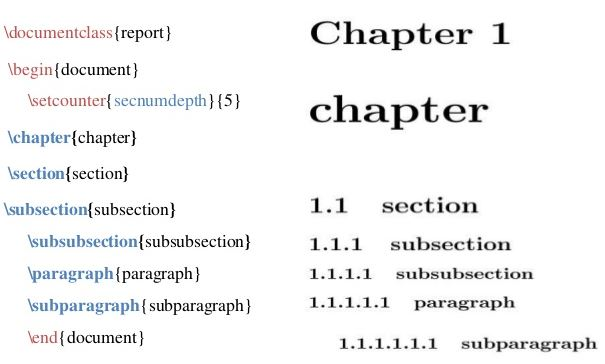
\includegraphics[width=0.50\textwidth]{gambar/dokumen}}
	\caption{dokumen}
	\label{dokumen}
\end{figure}

\vspace{50pt}
\hspace{0.50in} Sedangkan dokumen kelas report dan book selain memiliki perintah-perintah di atas memiliki juga perintah :
 \par
{\fontsize{10pt}{10pt}\selectfont  $  \setminus  $part $  \{  $... $  \}  $}
 \par
\vspace{9pt}

{\fontsize{10pt}{10pt}\selectfont  $  \setminus  $chapter $  \{  $... $  \}  $}
 \par
\vspace{9pt}
{\fontsize{10pt}{10pt}\selectfont  $  \setminus  $frontmatter}
 \par
\vspace{9pt}
{\fontsize{10pt}{10pt}\selectfont  $  \setminus  $mainmatter}
 \par
\vspace{9pt}
{\fontsize{10pt}{10pt}\selectfont  $  \setminus  $backmatter}
 \par
\vspace{12pt}
\hspace{0.50in} Argumen yang diberikan pada perintah-perintah ini adalah nama bab, subbab, dll. Dalam naskah buku yang dituliskan dengan kelas dokumen book, fronmatter digunakan untuk menandai halaman judul, daftar isi, kata pengantar, daftar gambar, dsb. Sedangkan mainmatter digunakan untuk menandai bagian tulisan utama, dan backmatter untuk menandai daftar pustaka, indeks, daftar istilah, dsb. Perintah  $  \setminus  $chapter,  $  \setminus  $section,  $  \setminus  $subsection, dan  $  \setminus  $subsubsection secara otomatis memberikan nomor pada nama bagian, bab, dsb. Jika nomor ini tidak diinginkan, perintah yang ekivalen adalah  $  \setminus  $chapter*,  $  \setminus  $section*,  $  \setminus  $subsection*, dan  $  \setminus  $subsubsection*.
 \par
\vspace{12pt}
\hspace{0.50in} Perintah bagian diberi nomor dan akan muncul dalam daftar isi dokumen. Paragraf tidak diberi nomor dan tidak akan ditampilkan dalam daftar isi. Berikut contoh output menggunakan bagian:
 \par
1 Section
 \par
~~ Hello World!
 \par
~~~~~ 1.1 Subsection
 \par
~~~~~~~~~~~~ Structuring a document is easy
 \par
\vspace{12pt}
\hspace{0.50in} Untuk mendapatkan hasil ini, Anda hanya perlu menambahkan beberapa baris ke program kami dari pelajaran 1:
 \par
 $  \setminus  $documentclass $  \{  $article $  \}  $
 \par
\vspace{12pt}
 $  \setminus  $title $  \{  $Title of my document $  \}  $
 \par
 $  \setminus  $date $  \{  $2013-09-01 $  \}  $
 \par
 $  \setminus  $author $  \{  $John Doe $  \}  $
 \par
\vspace{12pt}
 $  \setminus  $begin $  \{  $document $  \}  $
 \par
\vspace{12pt}
 $  \setminus  $maketitle
 \par
 $  \setminus  $pagenumbering $  \{  $gobble $  \}  $
 \par

 $  \setminus  $newpage
 \par
 $  \setminus  $pagenumbering $  \{  $arabic $  \}  $
 \par
\vspace{12pt}
 $  \setminus  $section $  \{  $Section $  \}  $
 \par
\vspace{12pt}
Hello World!
 \par
\vspace{12pt}
 $  \setminus  $subsection $  \{  $Subsection $  \}  $
 \par
\vspace{12pt}
Structuring a document is easy!
 \par
\vspace{12pt}
 $  \setminus  $end $  \{  $document $  \}  $
 \par
\vspace{14pt}
Gambar berikut menunjukkan struktur hirarkis dari semua elemen:
 \par
1. Section
 \par
~~~ Hello World
 \par
~~~~ 1.1 Subsection
 \par
~~~~~~~~~~ Structuring a document is easy!
 \par
~~~~~~~~~ 1.1 Subsection
 \par
~~~~~~~~~~~~~~~ More Text
 \par
~~~~~~~~~~~~~~~ Paragraph ~~~~~~~~~~~~ Some more text
 \par
~~~~~~~~~~~~~~~ Subparagraph ~~~~~~~ Even more text \par
2. Another Section
 \par
\hspace{0.50in} Saya telah menggunakan kode berikut untuk mendapatkan output ini:
 \par
 $  \setminus  $documentclass $  \{  $article $  \}  $
 \par
\vspace{12pt}
 $  \setminus  $begin $  \{  $document $  \}  $
 \par
\vspace{12pt}
 $  \setminus  $section $  \{  $Section $  \}  $
 \par
\vspace{12pt}
Hello World!
 \par
\vspace{12pt}
 $  \setminus  $subsection $  \{  $Subsection $  \}  $
 \par
\vspace{12pt}
Structuring a document is easy!
 \par
\vspace{12pt}
 $  \setminus  $subsubsection $  \{  $Subsubsection $  \}  $
 \par
\vspace{12pt}
More text.
 \par
\vspace{12pt}
 $  \setminus  $paragraph $  \{  $Paragraph $  \}  $
 \par
\vspace{12pt}
Some more text.
 \par
\vspace{12pt}
 $  \setminus  $subparagraph $  \{  $Subparagraph $  \}  $
 \par
\vspace{12pt}
Even more text.
 \par
\vspace{12pt}
 $  \setminus  $section $  \{  $Another section $  \}  $
 \par
\vspace{12pt}
 $  \setminus  $end $  \{  $document $  \}  $
 \par
\vspace{12pt}
\vspace{12pt}
Contoh struktur dokumen berkelas article dan book :
 \par
{\fontsize{10pt}{10pt}\selectfont  $  \setminus  $documentclass $  \{  $article $  \}  $}
 \par
\vspace{10pt}
{\fontsize{10pt}{10pt}\selectfont  $  \setminus  $usepackage $  \{  $... $  \}  $}
 \par
\vspace{10pt}
{\fontsize{10pt}{10pt}\selectfont  $  \setminus  $begin $  \{  $document $  \}  $}
 \par
\vspace{10pt}
{\fontsize{10pt}{10pt}\selectfont  $  \setminus  $maketitle}
 \par
\vspace{10pt}
{\fontsize{10pt}{10pt}\selectfont  $  \setminus  $section $  \{  $... $  \}  $}
 \par
\vspace{10pt}
{\fontsize{10pt}{10pt}\selectfont  $  \setminus  $section $  \{  $... $  \}  $}
 \par
\vspace{10pt}
{\fontsize{10pt}{10pt}\selectfont  $  \setminus  $subsection $  \{  $... $  \}  $}
 \par
\vspace{10pt}
{\fontsize{10pt}{10pt}\selectfont  $  \setminus  $subsubsection $  \{  $... $  \}  $}
 \par
\vspace{10pt}
{\fontsize{10pt}{10pt}\selectfont  $  \setminus  $section}
 \par
\vspace{10pt}
{\fontsize{10pt}{10pt}\selectfont  $  \setminus  $end $  \{  $document $  \}  $}
 \par
\vspace{12pt}
\hspace{0.50in} LaTeX dapat menyusun dokumen menjadi beberapa bagian dengan sangat mudah. Hal ini karena LaTeX memiliki format yang konsisten di seluruh kertas. Berikut perintah-perintah latex, seperti:
 \begin{itemize}
\item part \par
\textit{part} berfungsi untuk membuat pembagian bab, biasanya dibuat dalam halaman yang terpisah. Adapun penggunaannya adalah sebagai berikut:

{\fontsize{10pt}{10pt}\selectfont ~~  $  \setminus  $part $  \{  $[Judul] $  \}  $}
 \par
\item chapter \par
\textit{chapter} merupakan bab utama yang memuat judul. Penggunaannya demikian:
\par
{\fontsize{10pt}{10pt}\selectfont ~~  $  \setminus  $chapter $  \{  $[Judul] $  \}  $}
\par
\item section \par
\textit{section} merupakan pasal dari suatu bab. Contoh penggunaannya adalah sebagai berikut:\
 \par
{\fontsize{10pt}{10pt}\selectfont ~~~  $  \setminus  $section $  \{  $[Judul] $  \}  $}
 \par
\item subsection \par
subsection \textit{subsection} berfungsi untuk membuat sub pasal atau pasal baru di bawah judul pasal.
 \par
{\fontsize{10pt}{10pt}\selectfont ~~  $  \setminus  $subsection $  \{  $Judul $  \}  $}
 \par
\textit{subsubsection} berfungsi untuk membuat sub pasal di bawahnya lagi dari sub pasal yang ada.
 \par
{\fontsize{10pt}{10pt}\selectfont ~~  $  \setminus  $subsubsection* $  \{  $Judul $  \}  $}
 \par
 \item paragraph \par
\textit{paragraph} berguna untuk membuat alinea kalimat, cara penggunaannya adalah sebagai berikut:
 \par
{\fontsize{10pt}{10pt}\selectfont ~~  $  \setminus  $paragraph $  \{  $kalimat $  \}  $}
 \par
\item subparagraph \par
\textit{subpragraph} berfungsi untuk membuat alinea baru di dalam alinea yang sudah ada. Cara penggunaannya adalah demikian:
 \par
{\fontsize{10pt}{10pt}\selectfont ~~  $  \setminus  $subparagraph $  \{  $kalimat $  \}  $}
 \par
 \vspace{12pt}
Contoh struktur dokumen berikut ini:
 \par
{\fontsize{10pt}{10pt}\selectfont  $  \setminus  $part $  \{  $Memulai LATEX $  \}  $  $  \%  $ ini adalah contoh penggunaan part}
 \par
{\fontsize{10pt}{10pt}\selectfont ~~~~~  $  \setminus  $chapter $  \{  $Menggunakan LATEX $  \}  $  $  \%  $ ini adalah contoh penggunaan chapter}
 \par
{\fontsize{10pt}{10pt}\selectfont ~~~~~~~~~~~  $  \setminus  $section $  \{  $Penggunaan Class dalam penulisan dokumen $  \}  $}
 \par
{\fontsize{10pt}{10pt}\selectfont  \hspace*{0.64in} ~  \hspace*{0.64in}  \hspace*{0.64in}  $  \%  $ ini adalah contoh penggunaan section}
 \par
{\fontsize{10pt}{10pt}\selectfont ~~~~~~~~~~~~~~~~ $  \setminus  $subsection $  \{  $Penyertaan Package $  \}  $  }
 \par
{\fontsize{10pt}{10pt}\selectfont  \hspace*{0.64in}  \hspace*{0.64in}  \hspace*{0.64in}  $  \%  $ ini adalah contoh penggunaan subsection}
 \par
{\fontsize{10pt}{10pt}\selectfont  \hspace*{0.64in}  \hspace*{0.64in}  \hspace*{0.64in}  $  \setminus  $paragraph $  \{  $Penyertaan package berguna untuk menambahkan fungsi }
 \par
{\fontsize{10pt}{10pt}\selectfont  \hspace*{0.64in}  \hspace*{0.64in}  \hspace*{0.64in} kedalam dokumen/naskah yang kita buat. Bentuk penulisannya }
 \par
{\fontsize{10pt}{10pt}\selectfont  \hspace*{0.64in}  \hspace*{0.64in}  \hspace*{0.64in} adalah sebagai berikut: $  \}  $}
 \par
{\fontsize{10pt}{10pt}\selectfont   \hspace*{0.64in}  \hspace*{0.64in}  \hspace*{0.64in}  \hspace*{0.64in}  $  \%  $ ini adalah contoh penggunaan paragraph}
 \par
\end{itemize}
\vspace{10pt}
\subsection{Komentar}
 \par
\hspace{0.50in} Fungsi dari komentar adalah untuk menampilkan catatan dari naskah yang telah Anda buat, namun tidak ditampilkan pada saat file dicetak. Contoh penggunaan nya adalah sebagai berikut:
 \par
{\fontsize{10pt}{10pt}\selectfont  $  \setminus  $documentclass[12pt,a4paper,oneside,bahasa,dvips] $  \{  $book $  \}  $}
 \par
{\fontsize{10pt}{10pt}\selectfont  $  \setminus  $begin $  \{  $document $  \}  $}
 \par
{\fontsize{10pt}{10pt}\selectfont Halo, ini adalah contoh penulisan menggunakan LaTeX.}
 \par
{\fontsize{10pt}{10pt}\selectfont ukuran font dari naskah ini adalah 12. Pencetakan akan menggunakan}
 \par
{\fontsize{10pt}{10pt}\selectfont kertas A4, yang akan dicetak dalam satu sisi. Naskah ini berbentuk bu}
 \par
{\fontsize{10pt}{10pt}\selectfont dan akan ditampilkan kedalam bahasa Indonesia.}
 \par
{\fontsize{10pt}{10pt}\selectfont komentar ini tidak akan ditampilkan pada saat dilakukan pencetakan}
 \par
{\fontsize{10pt}{10pt}\selectfont naskah.}
 \par
{\fontsize{10pt}{10pt}\selectfont  $  \setminus  $end $  \{  $document $  \}  $}
 \par
\subsection{Membuat Judul Dokumen}
 \par
Untuk judul dokumen, perintahnya adalah sebagai berikut:
 \par
{\fontsize{10pt}{10pt}\selectfont  $  \setminus  $title $  \{  $ $  \}  $}
 \par
{\fontsize{10pt}{10pt}\selectfont  $  \setminus  $maketitle}
 \par
\vspace{12pt}
Adapun contohnya adalah sebagai berikut:
 \par
{\fontsize{10pt}{10pt}\selectfont  $  \setminus  $documentclass[12pt,a4paper,oneside,bahasa,dvips] $  \{  $book $  \}  $}
 \par
{\fontsize{10pt}{10pt}\selectfont  $  \setminus  $title $  \{  $Membuat Dokumen dengan  $  \setminus  $LaTeX $  \{  $ $  \}  $ $  \}  $}
 \par
{\fontsize{10pt}{10pt}\selectfont  $  \setminus  $begin $  \{  $document $  \}  $}
 \par
{\fontsize{10pt}{10pt}\selectfont  $  \setminus  $maketitle}
 \par
\vspace{10pt}
{\fontsize{10pt}{10pt}\selectfont Halo, ini adalah contoh penulisan menggunakan LaTeX, dengan ukuran font Pencetakan akan menggunakan kertas A4, yang akan dicetak dalam satu sis Naskah ini berbentuk buku dan akan ditampilkan kedalam bahasa Indonesia judul akan ditampilkan secara otomatis pada awal dokumen ketika dokumen dikonversi ke format DVI,HTML, ataupun PDF.  $  \setminus  $end $  \{  $document $  \}  $} 

\subsection{Memisahkan Baris} \par
Untuk memisahkan baris, Anda bisa menggunakan perintah sebagai berikut: \par
 $  \setminus  $ $  \setminus  $ \par
atau \par
{\fontsize{10pt}{10pt}\selectfont  $  \setminus  $newline} \par
\vspace{12pt}
Adapun contoh penggunaannya adalah demikian: \par
Contoh 1: \par
{\fontsize{10pt}{10pt}\selectfont  $  \setminus  $documentclass[12pt,a4paper,oneside,bahasa,dvips] $  \{  $book $  \}  $} \par
{\fontsize{10pt}{10pt}\selectfont  $  \setminus  $begin $  \{  $document $  \}  $} \par
\vspace{10pt}
{\fontsize{10pt}{10pt}\selectfont Halo, ini adalah contoh penulisan menggunakan LaTeX, dengan ukuran font Pencetakan akan menggunakan kertas A4, yang akan dicetak dalam satu sis Naskah ini berbentuk buku dan akan ditampilkan kedalam bahasa Indonesia} \par
\vspace{10pt}
{\fontsize{10pt}{10pt}\selectfont Tulisan ini akan ditampilkan dengan penambahan satu baris.} \par
{\fontsize{10pt}{10pt}\selectfont  $  \setminus  $end $  \{  $document $  \}  $} \par
\vspace{10pt}
Contoh 2: \par
{\fontsize{10pt}{10pt}\selectfont  $  \setminus  $documentclass[12pt,a4paper,oneside,bahasa,dvips] $  \{  $book $  \}  $} \par
{\fontsize{10pt}{10pt}\selectfont  $  \setminus  $begin $  \{  $document $  \}  $} \par
\vspace{10pt}
{\fontsize{10pt}{10pt}\selectfont Halo, ini adalah contoh penulisan menggunakan LaTeX, dengan ukuran font Pencetakan akan menggunakan kertas A4, yang akan dicetak dalam satu sis Naskah ini berbentuk buku dan akan ditampilkan kedalam bahasa Indonesia} \par
\vspace{10pt}
{\fontsize{10pt}{10pt}\selectfont  $  \setminus  $linebreak} \par
{\fontsize{10pt}{10pt}\selectfont Tulisan ini akan ditampilkan dengan penambahan satu baris.} \par

{\fontsize{10pt}{10pt}\selectfont  $  \setminus  $end $  \{  $document $  \}  $}
 \par

\subsection{Berpindah Halaman}
 \par
Untuk berpindah halaman, Anda bisa menggunakan perintah sebagai berikut: \par
\begin{equation}
newpage
\end{equation}

\vspace{9pt}
Contohnya adalah sebagai berikut \par
{\fontsize{10pt}{10pt}\selectfont  $  \setminus  $documentclass[12pt,a4paper,oneside,bahasa,dvips] $  \{  $book $  \}  $} \par
{\fontsize{10pt}{10pt}\selectfont  $  \setminus  $title $  \{  $Membuat Dokumen dengan  $  \setminus  $LaTeX $  \{  $ $  \}  $ $  \}  $} \par
{\fontsize{10pt}{10pt}\selectfont  $  \setminus  $author $  \{  $R. Kresno Aji (masaji@ai.co.id) $  \}  $} \par
{\fontsize{10pt}{10pt}\selectfont  $  \setminus  $date $  \{  $17 Agustus 2004 $  \}  $} \par
{\fontsize{10pt}{10pt}\selectfont  $  \setminus  $begin $  \{  $document $  \}  $} \par
{\fontsize{10pt}{10pt}\selectfont  $  \setminus  $maketitle} \par
\vspace{10pt}
{\fontsize{10pt}{10pt}\selectfont Halo, ini adalah contoh penulisan menggunakan LaTeX, dengan ukuran font Pencetakan akan menggunakan kertas A4, yang akan dicetak dalam satu sis Naskah ini berbentuk buku dan akan ditampilkan kedalam bahasa Indonesia judul akan ditampilkan secara otomatis pada awal dokumen ketika dokumen dikonversi ke format DVI,HTML, ataupun PDF.} \par
\vspace{10pt}
{\fontsize{10pt}{10pt}\selectfont  $  \setminus  $newpage} \par
{\fontsize{10pt}{10pt}\selectfont  $  \setminus  $chapter $  \{  $Halaman Baru $  \}  $} \par
{\fontsize{10pt}{10pt}\selectfont  $  \setminus  $end $  \{  $document $  \}  $} \par

\subsection{Environtment} \par
LATEX menyediakan environmen yang berupa: \par
* Itemize \par
~~ berfungsi untuk membuat daftar yang tidak memiliki urutan. \par
* Enumerate \par
~~ berfungsi untuk membuat daftar yang berurutan. \par
* Flushleft \par
~~ untuk membuat kalimat rata kiri. \par
* Center \par
~~ berfungsi untuk membuat kalimat dengan format center. \par
* Flushright \par
~~ berfungsi untuk membuat kalimat rata kanan. \par
* Footnote \par
~~ berfungsi untuk membuat catatan kaki. \par
* Verbatim \par
~~ berfungsi untuk membuat kalimat / karakter yang ditulis \par
* Table
 \par
~~ berfungsi untuk membuat tabel.  \par 
\begin{enumerate}
\item  Pembuatan daftar berurutan \par
Untuk membuat daftar yang berurutan, Anda bisa menggunakan perintah berikut ini: \par
{\fontsize{10pt}{10pt}\selectfont  $  \setminus  $begin $  \{  $enumerate $  \}  $} \par
{\fontsize{10pt}{10pt}\selectfont  $  \setminus  $item} \par
{\fontsize{10pt}{10pt}\selectfont  $  \setminus  $end $  \{  $enumerate $  \}  $} \par
\vspace{12pt}
Contohnya adalah demikian: \par
{\fontsize{10pt}{10pt}\selectfont  $  \setminus  $documentclass[12pt,a4paper,oneside,bahasa,dvips] $  \{  $book $  \}  $} \par
{\fontsize{10pt}{10pt}\selectfont  $  \setminus  $begin $  \{  $document $  \}  $} \par
\vspace{10pt}
{\fontsize{10pt}{10pt}\selectfont Halo, ini adalah contoh penulisan menggunakan LaTeX, dengan ukuran font Pencetakan akan menggunakan kertas A4, yang akan dicetak dalam satu sis Naskah ini berbentuk buku dan akan ditampilkan kedalam bahasa Indonesia Daftar secara berurutan akan ditampilkan secara otomatis pada awal {\fontsize{9pt}{9pt}\selectfont dokumen ketika dokumen dikonversi ke format DVI,HTML, ataupun PDF.}} \par
\vspace{12pt}
{\fontsize{10pt}{10pt}\selectfont Pada bab ini, kita akan membahas:} \par
{\fontsize{10pt}{10pt}\selectfont  $  \setminus  $begin $  \{  $enumerate $  \}  $} \par
{\fontsize{10pt}{10pt}\selectfont  $  \setminus  $item item satu} \par
{\fontsize{10pt}{10pt}\selectfont  $  \setminus  $item item dua} \par
{\fontsize{10pt}{10pt}\selectfont  $  \setminus  $end $  \{  $enumerate $  \}  $} \par
{\fontsize{10pt}{10pt}\selectfont  $  \setminus  $end $  \{  $document $  \}  $} \par
\vspace{10pt}
\noindent 
\item Penggunaan rata kiri, rata kanan dan center \par
\noindent 
~~~~ Untuk membuat dokumen LATEX menjadi rata kiri perintahnya adalah demikian: \par
{\fontsize{10pt}{10pt}\selectfont  $  \setminus  $begin $  \{  $flushleft $  \}  $} \par
{\fontsize{10pt}{10pt}\selectfont [kalimat]} \par
{\fontsize{10pt}{10pt}\selectfont  $  \setminus  $end $  \{  $flushleft $  \}  $} \par
\vspace{12pt}
Contohnya adalah sebagai berikut: \par
{\fontsize{10pt}{10pt}\selectfont  $  \setminus  $documentclass[12pt,a4paper,oneside,bahasa,dvips] $  \{  $book $  \}  $} \par
{\fontsize{10pt}{10pt}\selectfont  $  \setminus  $begin $  \{  $document $  \}  $} \par
{\fontsize{10pt}{10pt}\selectfont  $  \setminus  $begin $  \{  $flushleft $  \}  $} \par
\vspace{9pt}
{\fontsize{10pt}{10pt}\selectfont Halo, ini adalah contoh penulisan menggunakan LaTeX, dengan ukuran font Pencetakan akan menggunakan kertas A4, yang akan dicetak dalam satu sis Naskah ini berbentuk buku dan akan ditampilkan kedalam bahasa Indonesia dan berada di sebelah kiri.} \par
\vspace{9pt}
{\fontsize{10pt}{10pt}\selectfont  $  \setminus  $end $  \{  $flushleft $  \}  $} \par
{\fontsize{10pt}{10pt}\selectfont  $  \setminus  $end $  \{  $document $  \}  $} \par
\vspace{12pt}
Untuk membuat dokumen LATEX menjadi rata kanan, perintahnya adalah demikian: \par
{\fontsize{10pt}{10pt}\selectfont  $  \setminus  $begin $  \{  $flushright $  \}  $} \par
{\fontsize{10pt}{10pt}\selectfont [kalimat]} \par
{\fontsize{10pt}{10pt}\selectfont  $  \setminus  $end $  \{  $flushright $  \}  $} \par
\vspace{12pt}
Contohnya adalah sebagai berikut: \par
{\fontsize{10pt}{10pt}\selectfont  $  \setminus  $documentclass[12pt,a4paper,oneside,bahasa,dvips] $  \{  $book $  \}  $} \par
{\fontsize{10pt}{10pt}\selectfont  $  \setminus  $begin $  \{  $document $  \}  $} \par
{\fontsize{10pt}{10pt}\selectfont  $  \setminus  $begin $  \{  $flushright $  \}  $} \par
\vspace{10pt}
{\fontsize{10pt}{10pt}\selectfont Halo, ini adalah contoh penulisan menggunakan LaTeX, dengan ukuran font Pencetakan akan menggunakan kertas A4, yang akan dicetak dalam satu sis Naskah ini berbentuk buku dan akan ditampilkan kedalam bahasa Indonesia dan terletak rata kanan.} \par
\vspace{10pt}
{\fontsize{10pt}{10pt}\selectfont  $  \setminus  $end $  \{  $flushright $  \}  $} \par
{\fontsize{10pt}{10pt}\selectfont  $  \setminus  $end $  \{  $document $  \}  $} \par
\vspace{10pt}
Untuk membuat dokumen LATEX menjadi center perintahnya adalah demikian: \par
{\fontsize{10pt}{10pt}\selectfont  $  \setminus  $begin $  \{  $center $  \}  $} \par
{\fontsize{10pt}{10pt}\selectfont [kalimat]} \par
{\fontsize{10pt}{10pt}\selectfont  $  \setminus  $end $  \{  $center $  \}  $} \par
\vspace{10pt}
Contohnya adalah sebagai berikut: \par
{\fontsize{10pt}{10pt}\selectfont  $  \setminus  $documentclass[12pt,a4paper,oneside,bahasa,dvips] $  \{  $book $  \}  $ \hspace*{0.5in} } \par
{\fontsize{10pt}{10pt}\selectfont  $  \setminus  $begin $  \{  $document $  \}  $} \par
{\fontsize{10pt}{10pt}\selectfont  $  \setminus  $begin $  \{  $center $  \}  $} \par
\vspace{9pt}
{\fontsize{10pt}{10pt}\selectfont Halo, ini adalah contoh penulisan menggunakan LaTeX, dengan ukuran font Pencetakan akan menggunakan kertas A4, yang akan dicetak dalam satu sis Naskah ini berbentuk buku dan akan ditampilkan kedalam bahasa Indonesia dan terletak center.} \par
\vspace{9pt}
{\fontsize{10pt}{10pt}\selectfont  $  \setminus  $end $  \{  $center $  \}  $} \par
{\fontsize{10pt}{10pt}\selectfont  $  \setminus  $end $  \{  $document $  \}  $} \par
\vspace{14pt}
\noindent 
\item Pembuatan footnote \par
Untuk pembuatan footnote pada dokumen LATEX, Anda bisa memberikan perintah sebagai berikut:  \par
\vspace{12pt}
{\fontsize{10pt}{10pt}\selectfont  $  \setminus  $footnote $  \{  $ ...  $  \}  $} \par
\vspace{12pt}
Contohnya adalah demikian: \par
{\fontsize{10pt}{10pt}\selectfont  $  \setminus  $documentclass[12pt,a4paper,oneside,bahasa,dvips] $  \{  $book $  \}  $} \par
{\fontsize{10pt}{10pt}\selectfont  $  \setminus  $begin $  \{  $document $  \}  $} \par
\vspace{12pt}
{\fontsize{10pt}{10pt}\selectfont Halo, ini adalah contoh penulisan menggunakan LaTeX, dengan ukuran font Pencetakan akan menggunakan kertas A4, yang akan dicetak dalam satu sis Naskah ini berbentuk buku dan akan ditampilkan kedalam bahasa Indonesia  $  \setminus  $footnote $  \{  $Ini adalah contoh penggunaan footnote $  \}  $} \par
\vspace{9pt}
{\fontsize{10pt}{10pt}\selectfont  $  \setminus  $end $  \{  $document $  \}  $} \par
\vspace{10pt}
\noindent 
\item  Penulisan apa adanya dengan verbatim \par
Seperti halnya pada penulisan dalam format HTML, dengan menggunakan tag < pre >. LATEX juga menyediakan fasilitas ini. Adapun formatnya adalah sebagai berikut: \par
begin $  \{  $verbatim $  \}  $ \par
[kalimat] \par
end $  \{  $verbatim $  \}  $ \par
\vspace{8pt}
\vspace{8pt}
Contohnya adalah sebagai berikut: \par
{\fontsize{10pt}{10pt}\selectfont  $  \setminus  $begin $  \{  $verbatim $  \}  $} \par
{\fontsize{10pt}{10pt}\selectfont  $  \setminus  $documentclass[12pt,a4paper,oneside,bahasa,dvips] $  \{  $book $  \}  $} \par
{\fontsize{10pt}{10pt}\selectfont  $  \setminus  $begin $  \{  $document $  \}  $} \par
\vspace{10pt}
{\fontsize{10pt}{10pt}\selectfont Pada bab ini, kita akan membahas:} \par
{\fontsize{10pt}{10pt}\selectfont  $  \setminus  $begin $  \{  $itemize $  \}  $} \par
{\fontsize{10pt}{10pt}\selectfont  $  \setminus  $item item satu} \par
{\fontsize{10pt}{10pt}\selectfont  $  \setminus  $item item dua} \par
{\fontsize{10pt}{10pt}\selectfont  $  \setminus  $end $  \{  $itemize $  \}  $} \par
{\fontsize{10pt}{10pt}\selectfont  $  \setminus  $end $  \{  $document $  \}  $} \par
{\fontsize{10pt}{10pt}\selectfont end $  \{  $verbatim $  \}  $} \par
\vspace{10pt}
{\fontsize{10pt}{10pt}\selectfont Maka jika dilakukan pencetakan, hasilnya akan tampak sebagai berikut:} \par
{\fontsize{10pt}{10pt}\selectfont Pada bab ini, kita akan membahas:} \par
{\fontsize{10pt}{10pt}\selectfont  $  \setminus  $begin $  \{  $itemize $  \}  $} \par
{\fontsize{10pt}{10pt}\selectfont  $  \setminus  $item item satu} \par
{\fontsize{10pt}{10pt}\selectfont  $  \setminus  $item item dua} \par
{\fontsize{10pt}{10pt}\selectfont  $  \setminus  $end $  \{  $itemize $  \}  $} \par
\vspace{10pt}
\noindent 
\item Pembuatan Tabel \par
 Untuk membuat tabel pada dokumen LATEX, perintahnya adalah sebagai berikut: \par
{\fontsize{10pt}{10pt}\selectfont  $  \setminus  $begin $  \{  $tabular $  \}  $} \par
{\fontsize{10pt}{10pt}\selectfont  $  \setminus  $end $  \{  $tabular $  \}  $} \par
\vspace{12pt}
Untuk jelasnya, Anda bisa meniru langkah di bawah ini: \par
{\fontsize{10pt}{10pt}\selectfont  $  \setminus  $hline} \par
{\fontsize{10pt}{10pt}\selectfont  $  \setminus  $begin $  \{  $tabular $  \}  $ $  \{  $ $  \vert  $c $  \vert  $c $  \vert  $c $  \vert  $ $  \}  $} \par
{\fontsize{10pt}{10pt}\selectfont No.  $  \&  $  $  \setminus  $bf Uraian  $  \&  $ Jumlah  $  \setminus  $ $  \setminus  $} \par
{\fontsize{10pt}{10pt}\selectfont  $  \setminus  $hline} \par
\begin{itemize}
\item {\fontsize{10pt}{10pt}\selectfont  $  \&  $ Pembelian alat-alat kantor  $  \&  $ Rp. 250.000  $  \setminus  $ $  \setminus  $  $  \setminus  $cline $  \{  $2-2 $  \}  $}\end{itemize}
 \par
{\fontsize{10pt}{10pt}\selectfont  $  \setminus  $hline} \par
{\fontsize{10pt}{10pt}\selectfont  $  \setminus  $end $  \{  $tabular $  \}  $} \par
\vspace{12pt}
\noindent 
\item Mengubah bentuk dan ukuran font \par
Ada beberapa mode perubahan font pada LATEX, seperti bisa Anda lihat pada penjelasan berikut ini:
 \par
\vspace{12pt}
Untuk memperkecil huruf, perintahnya adalah demikian: \par
 $  \setminus  $small \par
\vspace{12pt}
Untuk memperbesar huruf, perintah sebagai berikut: \par
{\fontsize{10pt}{10pt}\selectfont  $  \setminus  $large} \par
{\fontsize{10pt}{10pt}\selectfont  $  \setminus  $LARGE} \par
{\fontsize{10pt}{10pt}\selectfont  $  \setminus  $Huge} \par
\vspace{12pt}
Contohnya adalah demikian: \par
\begin{verbatim}
\documentclass[12pt] {article} 
\begin {document} 
\end {document}
\end{verbatim}
\vspace{8pt}
\item Membuat daftar pustaka \par
Akhir dari pembuatan dokumen atau naskah ilmiah adalah dengan membuat daftar pustaka atau referensi. Pada LaTeX, hal ini sudah tersedia. Anda hanya perlu menggunakannya saja. Adapun perintahnya adalah sebagai berikut: \par
{\fontsize{10pt}{10pt}\selectfont  $  \setminus  $bibliographystyle $  \{  $plain $  \}  $} \par
{\fontsize{10pt}{10pt}\selectfont  $  \setminus  $begin $  \{  $thebibliography $  \}  $ $  \{  $Refference $  \}  $} \par
{\fontsize{10pt}{10pt}\selectfont  $  \setminus  $bibitem} \par
{\fontsize{10pt}{10pt}\selectfont  $  \setminus  $end $  \{  $thebibliography $  \}  $} \par
\vspace{12pt}
Untuk jelasnya, Anda bisa melihat contoh di bawah ini: \par
\begin{verbatim}
\bibliographystyle {plain}
\begin {thebibliography} {Refference}
\bibitem A Guide to LaTex}
\end {thebibliography} 
\end{verbatim}
\end{enumerate}


\chapter{Packages Explained}

\chapter{Typesetting Math in Latex}
\sloppy
 \hspace*{0.5in} Latex Adalah Sebuah alat yang sangat kuat untuk typesetting pada umumnya dan untuk typesetting matematika masuk tertentu. Namun, terlepas dari kekuatannya, masih banyak cara untuk menghasilkannya hasil yang lebih baik atau kurang bagus. Panduan ini menawarkan beberapa trik dan petunjuk yang mudah-mudahan akan dilakukan mengarah ke yang pertama Perhatikan bahwa manual ini tidak mengklaim untuk memberikan yang terbaik atau satu-satunya solusi. Tujuannya adalah untuk memberi beberapa aturan yang bisa diikuti dengan mudah dan itu akan memimpin ke tata letak yang baik dari semua persamaan dalam sebuah dokumen. Hal ini diasumsikan bahwa pembaca memiliki sudah menguasai dasar-dasar Latex \par
\noindent 
\vspace{12pt}
\noindent 
\vspace{12pt}
\noindent 
Bagaimana~persamaan typeset di  Sebuah Latex file sumber dari manual ini. \par
\noindent 
\vspace{12pt}
\noindent 
 dot $  \_  $emacs : perintah untuk disertakan dalam file preferensi Emacs (.emacs) \par
\noindent 
 IEEEtrantools.sty [2015/08/26 V1.5 oleh Michael Shell]: paket yang dibutuhkan untuk IEEEeqnarray-lingkungan Hidup. \par
\noindent 
 IEEEtran.cls [2015/08/26 V1.8b oleh Michael Shell]: Latex dalam format IEEE. \par
\noindent 
 IEEEtran $  \_  $HOWTO.pdf [2015/08]: manual resmi dari IEEEtran-kelas. Bagian tentang IEEEeqnarray dadjustwidthukan di Appendix F. Perhatikan itu IEEEtran.cls dan IEEEtrantools.sty disediakan secara otomatis oleh siapapun up-to-date.\
 \par
\noindent 
\vspace{12pt}
\noindent 
 \hspace*{0.5in} Struktur dokumen ini adalah sebagai berikut. Kami memperkenalkan persamaan yang paling dasar di Bagian 2; Bagian 3 kemudian menjelaskan beberapa kemungkinan reaksi pertama ketika sebuah persamaan terlalu panjang Bagian terpenting dari manual ini tercantum dalam Bagian 4 dan 5: disana kita perkenalkan yang bertenaga IEEEeqnarray lingkungan yang harus digunakan masuk apapun bukan meluruskan atau eqnarray.Dalam Bagian 6 beberapa masalah yang lebih maju dan solusi yang mungkin dibahas, dan Bagian 7 berisi beberapa petunjuk dan trik tentang editor Emacs. Akhirnya, Bagian 8 membuat beberapa saran tentang beberapa simbol matematika khusus yang tidak dapat dengan mudah dadjustwidthukan di Latex. \par
\noindent 
perintah akan diatur masuk font mesin tik .RHS berdiri untuk sisi kanan, yaitu, semua istilah di sebelah kanan tanda persamaan (atau ketidaks etaraan).Demikian pula,LHS berdiri untuk sisi kiri, yaitu, semua istilah di sebelah kiri tanda persamaan.Untuk menyederhanakan bahasa kita, kita biasanya akan membicarakannya persamaan. Jelas, typesetting tidak berubah jika sebuah ekspresi sebenarnya adalah ketidaksetaraan. Dokumen ini dilengkapi dengan beberapa file tambahan yang mungkin bisa membantu. \par
\noindent 
 \hspace*{0.5in} Kekuatan utama sebuah LATEX tentang tata bahasa matematika didasarkan pada \par
\noindent 
Paket amsmath. Setiap distribusi SEBUAH LATEX akan datang dengan paket ini \par
\noindent 
disertakan, jadi Anda hanya perlu memastikan bahwa baris berikut disertakan dalam header dokumen anda: \par
\noindent 
\vspace{10pt}
\noindent 
 $  \setminus  $usepackage $  \{  $amsmath $  \}  $ \par
\noindent 
\vspace{12pt}
\noindent 
 $  \setminus  $begin $  \{  $equation $  \}  $ \par
\vspace{12pt}
\noindent 
a = b + c \par
\vspace{12pt}
\noindent 
 $  \setminus  $end $  \{  $equation $  \}  $ \par
\vspace{12pt}
\noindent 
Jika seseorang tidak ingin memiliki nomor persamaan, * -version digunakan: \par
\vspace{12pt}
\noindent 
 $  \setminus  $begin $  \{  $equation* $  \}  $ \par
\vspace{12pt}
\noindent 
a = b + c \par
\vspace{12pt}
\noindent 
 $  \setminus  $end $  \{  $equation* $  \}  $ \par
\vspace{12pt}
\noindent 
Semua kemungkinan lain untuk typesetting persamaan sederhana memiliki kelemahan: \par
\noindent 
  $ \bullet $Itu tampilan matematis lingkungan tidak menawarkan penomoran persamaan. Untuk menambahkan atau re-pindahkan "*" dipersamaan lingkungan jauh lebih fleksibel.
 \par
\noindent 

 Perintah seperti  $  \$  $ $  \$  $ ...  $  \$  $ $  \$  $ , $  \setminus  $ [...  $  \setminus  $], dll, memiliki kelemahan tambahan itu kode sumbernya sangat mudah dibaca. Bahkan,  $  \$  $ $  \$  $ ...  $  \$  $ $  \$  $ salah: Jarak vertikal setelah persamaan terlalu besar dalam situasi tertentu. \par
\vspace{12pt}
\noindent 
\textbf{Persamaan Tunggal yang Terlalu Panjang: multline} \par
\vspace{12pt}
\noindent 
 \hspace*{0.5in} Jika sebuah persamaan terlalu panjang, kita harus membungkusnya entah bagaimana. Sayangnya, dibungkus equa-Tions biasanya kurang mudah dibaca daripada yang tidak terbungkus. Untuk meningkatkan keterbacaan, Kita harus mengikuti peraturan tertentu tentang bagaimana melakukan pembungkus: \par
\noindent 

 Secara umum, seseorang harus selalu membungkus sebuah persamaan \par
\noindent 
 Sebelum tanda kesetaraan atau seorang operator \par
\noindent 
 Bungkus sebelum tanda kesetaraan lebih baik dibungkus sebelum operator. \par
Bungkus sebelum operator plus atau minus lebih baik dibungkus sebelum aperkalian-operator \par
\noindent 
 Jenis bungkus lainnya harus dihindari jika memungkinkan.
 \par
\vspace{12pt}
\vspace{12pt}
\noindent 
Cara termudah untuk mencapai pembungkus seperti itu adalah penggunaan \par
\noindent 
multline-lingkungan Hidup: \par
\vspace{12pt}
\noindent 
 $  \setminus  $begin $  \{  $multline $  \}  $ \par
\vspace{12pt}
\noindent 
a + b + c + d + e + f \par
\vspace{12pt}
\noindent 
+ g + h + i \par
\vspace{12pt}
\noindent 
 $  \setminus  $ $  \setminus  $ \par
\vspace{12pt}
\noindent 
= j + k + l + m + n \par
\vspace{12pt}
\noindent 
 $  \setminus  $end $  \{  $multline $  \}  $ \par
\vspace{12pt}
\noindent 
 \hspace*{0.5in} Perbedaannya dengan persamaan lingkungan adalah bahwa break-line sewenang-wenang (atau juga beberapa baris-istirahat) dapat diperkenalkan. Hal ini dilakukan dengan meletakkan a $  \setminus  $ $  \setminus  $ di tempat itu dimana persamaan perlu dibungkus. Demikian pula untuk persamaan* ada juga amultline *-versi untuk mencegah a nomor persamaan Namun, meski mudah digunakan, seringkali IEEEeqnarray lingkungan akan menghasilkan hasil yang lebih baik. Terutama, pertimbangkan situasi umum berikut ini: \par
\vspace{12pt}
\vspace{12pt}
\noindent 
 $  \setminus  $begin $  \{  $equation $  \}  $ \par
\vspace{12pt}
\noindent 
a = b + c + d + e + f \par
\vspace{12pt}
\noindent 
+ g + h + i + j \par
\vspace{12pt}
\noindent 
+ k + l + m + n + o + p \par
\vspace{12pt}
\noindent 
 $  \setminus  $label $  \{  $eq:equation $  \_  $too $  \_  $long $  \}  $ \par
\vspace{12pt}
\noindent 
 $  \setminus  $end $  \{  $equation $  \}  $ \par
\vspace{12pt}
\vspace{16pt}
\noindent 
Disini RHS terlalu panjang untuk muat di satu baris. Itu Multline - lingkungan sekarang akan menghasilkan pengikut: \par
\vspace{12pt}
\noindent 
 $  \setminus  $begin $  \{  $multline $  \}  $ \par
\vspace{12pt}
\noindent 
a = b + c + d + e + f \par
\vspace{12pt}
\noindent 
+ g + h + i + j  $  \setminus  $ $  \setminus  $ \par
\vspace{12pt}
\noindent 
+ k + l + m + n + o + p \par
\vspace{12pt}
\noindent 
 $  \setminus  $end $  \{  $multline $  \}  $ \par
\vspace{12pt}
\vspace{16pt}
\noindent 
 \hspace*{0.5in} Hal ini tentunya jauh lebih baik dari (3), namun memiliki kelemahan yaitu persamaan Tanda kehilangan kepentingannya yang lebih kuat dari operator plus di depan. Lebih baik Solusi disediakan oleh IEEEeqnarray - lingkungan yang akan dibahas secara detail. \par
\vspace{12pt}
\noindent 
 $  \setminus  $begin $  \{  $IEEEeqnarray $  \}  $ $  \{  $rCl $  \}  $ \par
\vspace{12pt}
\noindent 
a  $  \&  $ =  $  \&  $ b + c + d + e + f \par
\vspace{12pt}
\noindent 
+ g + h + i + j  $  \setminus  $nonumber $  \setminus  $ $  \setminus  $ \par
\vspace{12pt}
\noindent 
 $  \&  $ $  \&  $ + $  \setminus  $> k + l + m + n + o + p \par
\vspace{12pt}
\noindent 
 $  \setminus  $label $  \{  $eq:dont $  \_  $use $  \_  $multline $  \}  $ \par
\vspace{12pt}
\noindent 
 $  \setminus  $end $  \{  $IEEEeqnarray $  \}  $ \par
\vspace{12pt}
\noindent 
 \hspace*{0.5in} Dalam hal ini baris kedua secara horizontal sejajar dengan baris pertama: + di depan k aku s tepatnya di bawah b , yaitu, RHS jelas terlihat kontras dengan persamaan LHS. Perhatikan juga itu multline salah memaksakan jarak minimum di sebelah kiri yang pertama garis bahkan jika tidak memiliki cukup ruang di sebelah kanan, menyebabkan persamaan yang tidak tersisip. Ini \par
\noindent 
Bahkan bisa mengarah pada tata letak yang sangat jelek dimana baris kedua berisi RHS dari sebuah persamaan sebenarnya ke kiri dari baris pertama yang berisi LHS: \par
\noindent 
 $  \setminus  $begin $  \{  $multline $  \}  $ \par
\vspace{12pt}
\noindent 
a + b + c + d + e + f + g \par
\vspace{12pt}
\noindent 
+ h + i + j  $  \setminus  $ $  \setminus  $ \par
\vspace{12pt}
\noindent 
= k + l + m + n + o + p + q \par
\vspace{12pt}
\noindent 
+ r + s + t + u \par
\vspace{12pt}
\noindent 
 $  \setminus  $end $  \{  $multline $  \}  $ \par
\noindent 
\vspace{16pt}
\noindent 
Sekali lagi ini terlihat jauh lebih baik menggunakan IEEEeqnarray : \par
\vspace{12pt}
\noindent 
 $  \setminus  $begin $  \{  $IEEEeqnarray $  \}  $ $  \{  $rCl $  \}  $ \par
\vspace{12pt}
\noindent 
 $  \setminus  $IEEEeqnarraymulticol $  \{  $3 $  \}  $ $  \{  $l $  \}  $ $  \{  $ $  \%  $ \par
\vspace{12pt}
\noindent 
a + b + c + d + e + f + g \par
\vspace{12pt}
\noindent 
+ h + i + j \par
\vspace{12pt}
\noindent 
 $  \}  $ $  \setminus  $nonumber $  \setminus  $ $  \setminus  $* $  \%  $ \par
\vspace{12pt}
\noindent 
 $  \&  $ =  $  \&  $ k + l + m + n + o + p + q \par
\vspace{12pt}
\noindent 
+ r + s + t + u  $  \setminus  $nonumber $  \setminus  $ $  \setminus  $* \par
\vspace{12pt}
\noindent 
 $  \setminus  $end $  \{  $IEEEeqnarray $  \}  $ \par
\vspace{12pt}
\vspace{12pt}
\noindent 
Kasus 1: Ekspresi bukanlah sebuah persamaan Jika ungkapan itu bukan persamaan, maksudnya, tidak ada tanda kesetaraan, maka tidak ada RHS atau LHS dan multline menawarkan solusi yang bagus: \par
\vspace{12pt}
\noindent 
 $  \setminus  $begin $  \{  $multline $  \}  $ \par
\vspace{12pt}
\noindent 
a + b + c + d + e + f  $  \setminus  $ $  \setminus  $ \par
\vspace{12pt}
\noindent 
+ g + h + i + j + k + l  $  \setminus  $ $  \setminus  $ \par
\vspace{12pt}
\noindent 
+ m + n + o + p + q \par
\vspace{12pt}
\noindent 
 $  \setminus  $end $  \{  $multline $  \}  $ \par
\vspace{12pt}
\noindent 
Kasus 2: Komentar tambaha n Jika ada komentar tambahan di akhir persamaan yang tidak sesuaibaris yang sama, maka komentar ini bisa dimasukkan ke baris berikutnya: \par
\vspace{12pt}
\noindent 
 $  \setminus  $begin $  \{  $multline $  \}  $ \par
\noindent 
a + b + c + d \par
\vspace{12pt}
\noindent 
= e + f + g + h,  $  \setminus  $quad  $  \setminus  $ $  \setminus  $ \par
\vspace{12pt}
\noindent 
 $  \setminus  $text $  \{  $for  $  \}  $ 0  $  \setminus  $le n \par
\vspace{12pt}
\noindent 
 $  \setminus  $le n $  \_  $ $  \{  $ $  \setminus  $textnormal $  \{  $max $  \}  $ $  \}  $ \par
\vspace{12pt}
\noindent 
 $  \setminus  $end $  \{  $multline $  \}  $ \par
\vspace{12pt}
\vspace{16pt}
\noindent 
Kasus 3: LHS terlalu panjang - RHS terlalu pendek Jika LHS dari satu persamaan terlalu panjang dan RHS sangat pendek, maka orang tidak dapat melakukannya Selesaikan persamaan di depan tanda kesetaraan seperti yang diinginkan, tapi seseorang terpaksa melakukannya di suatu tempat di LHS. Dalam hal ini seseorang tidak dapat secara baik menjaga pemisahan alami \par
\noindent 
LHS dan RHS pula dan multline menawarkan solusi yang bagus: \par
\vspace{12pt}
\vspace{12pt}
\noindent 
 $  \setminus  $begin $  \{  $multline $  \}  $ \par
\vspace{12pt}
\noindent 
a + b + c + d + e + f \par
\vspace{12pt}
\noindent 
+ g  $  \setminus  $ $  \setminus  $+ h + i + j \par
\vspace{12pt}
\noindent 
+ k + l = m \par
\vspace{12pt}
\noindent 
 $  \setminus  $end $  \{  $multline $  \}  $ \par
\vspace{12pt}
\noindent 
Kasus 4: Istilah di RHS tidak boleh dibagi Berikut ini adalah kasus khusus (dan agak jarang): LHS akan cukup pendek dan / atau RHS cukup lama untuk membungkus persamaan dengan cara seperti ditunjukkan pada (5), yaitu, ini biasanya akan meminta IEEEeqnarray -lingkungan Hidup. Namun, istilah di RHS adalah sebuah entitas yang kita anggap tidak akan terbelah, tapi terlalu panjang untuk disesuaikan: \par
\vspace{12pt}
\noindent 
 $  \setminus  $begin $  \{  $multline $  \}  $ \par
\vspace{12pt}
\noindent 
h $  \string^  $ $  \{  $- $  \}  $(X $  \vert  $Y)  $  \setminus  $le  $  \setminus  $frac $  \{  $n+1 $  \}  $ $  \{  $e $  \}  $ \par
\vspace{12pt}
\noindent 
- h(X $  \vert  $Y) \par
\vspace{12pt}
\noindent 
 $  \setminus  $ $  \setminus  $ \par
\noindent 
+  $  \setminus  $int p(y)  $  \setminus  $log  $  \setminus  $left( \par
\vspace{12pt}
\noindent 
 $  \setminus  $frac $  \{  $ $  \setminus  $mathsf $  \{  $E $  \}  $ $  \setminus  $bigl[ $  \vert  $X $  \vert  $ $  \string^  $2 \par
\vspace{12pt}
\noindent 
 $  \setminus  $big $  \vert  $ Y=y $  \setminus  $bigr] $  \}  $ $  \{  $n $  \}  $ \par
\vspace{12pt}
\noindent 
 $  \setminus  $right)  $  \setminus  $dd y \par
\noindent 
 $  \setminus  $end $  \{  $multline $  \}  $ \par
\noindent 
Dalam contoh ini integral pada RHS terlalu panjang, tapi tidak boleh dibagi untuk read- kemampuan. Perhatikan bahwa bahkan dalam kasus ini, mungkin saja untuk menemukan solusi berbeda berdasarkan IEEEeqnarray -lingkungan Hidup: \par
\vspace{12pt}
\vspace{12pt}
\noindent 
 $  \setminus  $begin $  \{  $IEEEeqnarray $  \}  $ $  \{  $rCl $  \}  $ \par
\vspace{12pt}
\noindent 
 $  \setminus  $IEEEeqnarraymulticol $  \{  $3 $  \}  $ $  \{  $l $  \}  $ $  \{  $ \par
\vspace{12pt}
\noindent 
h $  \string^  $ $  \{  $- $  \}  $(X $  \vert  $Y) \par
\vspace{12pt}
\noindent 
 $  \}  $ $  \setminus  $nonumber $  \setminus  $ $  \setminus  $ $  \setminus  $quad \par
\vspace{12pt}
\noindent 
 $  \&  $  $  \setminus  $le  $  \&  $  $  \setminus  $frac $  \{  $n+1 $  \}  $ $  \{  $e $  \}  $ \par
\vspace{12pt}
\noindent 
- h(X $  \vert  $Y)  $  \setminus  $nonumber $  \setminus  $ $  \setminus  $ \par
\vspace{12pt}
\noindent 
 $  \&  $ $  \&  $ +  $  \setminus  $int p(y)  $  \setminus  $log  $  \setminus  $left( \par
\vspace{12pt}
\noindent 
 $  \setminus  $frac $  \{  $ $  \setminus  $mathsf $  \{  $E $  \}  $ $  \setminus  $bigl[ $  \vert  $X $  \vert  $ $  \string^  $2 \par
\vspace{12pt}
\noindent 
 $  \setminus  $big $  \vert  $ Y=y $  \setminus  $bigr] $  \}  $ $  \{  $n $  \}  $ \par
\vspace{12pt}
\noindent 
 $  \setminus  $right)  $  \setminus  $dd y \par
\vspace{12pt}
\noindent 
 $  \setminus  $nonumber $  \setminus  $ $  \setminus  $* \par
\vspace{12pt}
\noindent 
 $  \setminus  $end $  \{  $IEEEeqnarray $  \}  $ \par
\vspace{12pt}
\vspace{12pt}
\noindent 
\textbf{Beberapa Persamaan: IEEEeqnarray} \par
\noindent 
 \hspace*{0.5in} Dalam situasi yang paling umum, kita memiliki urutan beberapa persamaan yang tidak sesuai ke satu baris Disini kita perlu bekerja dengan kesejajaran horizontal untuk menjaga array persamaan dalam struktur yang bagus dan mudah dibaca. Sebelum kami memberikan saran tentang cara melakukannya, kami mulai dengan beberapa buruk contoh yang menunjukkan kelemahan terbesar dari solusi umum. 4.1 Masalah dengan perintah tradisional Untuk mengelompokkan beberapa persamaan, meluruskan -lingkungan Hidup 4 bisa digunakan : \par
\vspace{12pt}
\noindent 
 $  \setminus  $begin $  \{  $align $  \}  $ \par
\vspace{12pt}
\noindent 
a  $  \&  $ = b + c  $  \setminus  $ $  \setminus  $ \par
\vspace{12pt}
\noindent 
 $  \&  $ = d + e \par
\vspace{12pt}
\noindent 
 $  \setminus  $end $  \{  $align $  \}  $ \par
\vspace{12pt}
\noindent 
Sementara ini terlihat rapi asalkan setiap persamaan sesuai dengan satu garis, pendekatan ini tidak Tidak bekerja lagi begitu satu baris terlalu panjang \par
\noindent 
 $  \setminus  $begin $  \{  $align $  \}  $ \par
\vspace{12pt}
\noindent 
a  $  \&  $ = b + c  $  \setminus  $ $  \setminus  $ \par
\vspace{12pt}
\noindent 
 $  \&  $ = d + e + f + g + h + i \par
\noindent 
  \par
\noindent 
+ j + k + l  $  \setminus  $nonumber $  \setminus  $ $  \setminus  $ \par
\vspace{12pt}
\noindent 
 $  \&  $ + m + n + o  $  \setminus  $ $  \setminus  $ \par
\vspace{12pt}
\noindent 
 $  \&  $ = p + q + r + s \par
\vspace{12pt}
\noindent 
 $  \setminus  $end $  \{  $align $  \}  $ \par
\vspace{12pt}
\noindent 
Disini + m harus di bawah d dan tidak di bawah tanda kesetaraan. Tentu saja, bisa saja tambahkan beberapa spasi, misalnya,  $  \setminus  $ hspace  $  \{  $... $  \}  $ , tapi ini tidak akan pernah menghasilkan pengaturan yang tepat (dan gaya pemrograman yang buruk!). Solusi yang lebih baik ditawarkan oleh eqnarray -lingkungan Hidup \par
\vspace{12pt}
\noindent 
 $  \setminus  $begin $  \{  $eqnarray $  \}  $ \par
\vspace{12pt}
\noindent 
a  $  \&  $ =  $  \&  $ b + c  $  \setminus  $ $  \setminus  $ \par
\vspace{12pt}
\noindent 
 $  \&  $ =  $  \&  $ d + e + f + g + h + i \par
\vspace{12pt}
\noindent 
+ j + k + l  $  \setminus  $nonumber $  \setminus  $ $  \setminus  $ \par
\vspace{12pt}
\noindent 
 $  \&  $ $  \&  $ + $  \setminus  $> m + n + o  $  \setminus  $ $  \setminus  $ \par
\vspace{12pt}
\noindent 
 $  \&  $ =  $  \&  $ p + q + r + s \par
\vspace{12pt}
\noindent 
 $  \setminus  $end $  \{  $eqnarray $  \}  $ \par
\noindent 
\vspace{16pt}
\noindent 
Itu eqnarray -lingkungan Hidup, 5 Namun, memiliki beberapa kelemahan yang sangat parah: \par
\noindent 
 Ruang di sekitar tanda-tanda kesetaraan terlalu besar. Terutama, memang begitu tidak itu sama seperti di multline – dan persamaan lingkungan: \par
\vspace{12pt}
\noindent 
 $  \setminus  $begin $  \{  $eqnarray $  \}  $ \par
\vspace{12pt}
\noindent 
a  $  \&  $ =  $  \&  $ a = a \par
\vspace{12pt}
\noindent 
 $  \setminus  $end $  \{  $eqnarray $  \}  $ \par
\vspace{12pt}
\noindent 
Ungkapan kadang tumpang tindih dengan angka persamaan meski ada akan cukup ruang di sebelah kiri: \par
\vspace{12pt}
\noindent 
 $  \setminus  $begin $  \{  $eqnarray $  \}  $ \par
\vspace{12pt}
\noindent 
a  $  \&  $ =  $  \&  $ b + c \par
\noindent 
 $  \setminus  $ $  \setminus  $ \par
\vspace{12pt}
\noindent 
 $  \&  $ =  $  \&  $ d + e + f + g + h $  \string^  $2 \par
\vspace{12pt}
\noindent 
+ i $  \string^  $2 + j \par
\vspace{12pt}
\noindent 
 $  \setminus  $label $  \{  $eq:faultyeqnarray $  \}  $ \par
\vspace{12pt}
\noindent 
 $  \setminus  $end $  \{  $eqnarray $  \}  $ \par
\vspace{12pt}
\noindent 
Itu eqnarray lingkungan menawarkan sebuah perintah  $  \setminus  $ lefteqn  $  \{  $... $  \}  $ yang bisa digunakan ketika LHS terlalu panjang: \par
\noindent 
\vspace{16pt}
\noindent 
 $  \setminus  $begin $  \{  $eqnarray $  \}  $ \par
\vspace{12pt}
\noindent 
 $  \setminus  $lefteqn $  \{  $a + b + c + d \par
\vspace{12pt}
\noindent 
+ e + f + g + h $  \}  $ $  \setminus  $nonumber $  \setminus  $ $  \setminus  $ \par
\vspace{12pt}
\noindent 
 $  \&  $ =  $  \&  $ i + j + k + l + m \par
\vspace{12pt}
\noindent 
 $  \setminus  $ $  \setminus  $ \par
\vspace{12pt}
\noindent 
 $  \&  $ =  $  \&  $ n + o + p + q + r + s \par
\vspace{12pt}
\noindent 
 $  \setminus  $end $  \{  $eqnarray $  \}  $ \par
\noindent 
\vspace{16pt}
\noindent 
Sayangnya, perintah ini salah: jika RHS terlalu pendek, arraynya tidak terpusat dengan benar \par
\noindent 
\vspace{16pt}
\noindent 
 $  \setminus  $begin $  \{  $eqnarray $  \}  $ \par
\vspace{12pt}
\noindent 
 $  \setminus  $lefteqn $  \{  $a + b + c + d \par
\vspace{12pt}
\noindent 
+ e + f + g + h $  \}  $ \par
\vspace{12pt}
\noindent 
 $  \setminus  $nonumber $  \setminus  $ $  \setminus  $ \par
\vspace{12pt}
\noindent 
 $  \&  $ =  $  \&  $ i + j \par
\vspace{12pt}
\noindent 
 $  \setminus  $end $  \{  $eqnarray $  \}  $ \par
\vspace{12pt}
\noindent 
Apalagi sangat rumit untuk mengubah kesejajaran horizontal dari persamaan tanda di baris kedua.  \par
\vspace{12pt}
\noindent 
Solusi:~penggunaan dasar IEEEeqnarray Itu IEEEeqnarray  Lingkungan adalah perintah yang sangat kuat dengan banyak pilihan. DiManual ini kami hanya akan memperkenalkan beberapa fungsi yang paling penting. Untuk informasi lebih lanjut kami lihat manual resmi Pertama-tama, agar bisa menggunakan IEEEeqnarray Lingkungan, seseorang perlu memasukkan paketnya IEEEtrantools Sertakan baris berikut di header dokumen Anda: \par
\vspace{12pt}
\vspace{12pt}
\noindent 
 $  \setminus  $usepackage $  \{  $IEEEtrantools $  \}  $ \par
\vspace{12pt}
\noindent 
Kekuatan IEEEeqnarray adalah kemungkinan menentukan jumlah kolom dalam array persamaan Biasanya, spesifikasi ini akan jadi  $  \{  $rCl $  \}  $, yaitu tiga kolom, yaitu Kolom pertama benar-dibenarkan, yang tengah berpusat dengan sedikit ruang lebih banyak t (oleh karena itu kita tentukan kapital C bukan huruf kecil c) dan kolom ketiga dibiarkan dibenarkan: \par
\vspace{12pt}
\noindent 
 $  \setminus  $begin $  \{  $IEEEeqnarray $  \}  $ $  \{  $rCl $  \}  $ \par
\vspace{12pt}
\noindent 
a  $  \&  $ =  $  \&  $ b + c \par
\vspace{12pt}
\noindent 
 $  \setminus  $ $  \setminus  $ \par
\vspace{12pt}
\noindent 
 $  \&  $ =  $  \&  $ d + e + f + g + h \par
\vspace{12pt}
\noindent 
+ i + j + k  $  \setminus  $nonumber $  \setminus  $ $  \setminus  $ \par
\vspace{12pt}
\noindent 
 $  \&  $ $  \&  $ + $  \setminus  $> l + m + n + o \par
\vspace{12pt}
\noindent 
 $  \setminus  $ $  \setminus  $ \par
\vspace{12pt}
\noindent 
 $  \&  $ =  $  \&  $ p + q + r + s \par
\vspace{12pt}
\noindent 
 $  \setminus  $end $  \{  $IEEEeqnarray $  \}  $ \par
\vspace{12pt}
\vspace{16pt}
\noindent 
 \hspace*{0.5in} Namun, kita bisa menentukan jumlah kolom yang dibutuhkan. Sebagai contoh,  $  \{  $c $  \}  $ akan memberi saja satu kolom (yang terpusat) atau  $  \{  $rCl "l $  \}  $akan menambahkan kolom keempat yang dibenarkan kiri itu bergeser ke kanan (jaraknya ditentukan oleh "), misalnya untuk spesifikasi tambahan.Apalagi disamping l,c,r,L,C,R untuk entri mode matematika, ada juga s,t,kamu untuk kiri, tengah, dan kanan. Dan spasi tambahan bisa jadi ditambahkan oleh. Dan /dan ? dan "dalam rangka meningkatkan ketertiban. 8 Rincian lebih lanjut tentang penggunaan IEEEeqnarrayakan diberikan di Bagian 5. Perhatikan bahwa berbeda dengan eqnarray ruang di sekitar tanda-tanda persamaan benar. \par
\vspace{20pt}
\noindent 
{\fontsize{14pt}{14pt}\selectfont \textbf{Sebuah komentar tentang konsistensi} \\} \par
\vspace{24pt}
\noindent 
Ada tiga isu lagi yang belum disebutkan sejauh ini, tapi itu mungkin penyebabnya ketidakkonsistenan saat ketiga lingkungan tersebut, persamaan, \par
\noindent 
multline, dan IEEEeqnarray, digunakan secara intermixedly: \par
\noindent 
 multline memungkinkan sebuah persamaan dimulai dari atas halaman, sementara persamaan dan IEEEeqnarray cobalah untuk meletakkan garis teks terlebih dahulu, sebelum persamaan dimulai. Bahkan, jarak sebelum dan sesudah lingkungan tidak persis sama persamaan,multline, dan IEEEeqnarray. \par
\noindent 
  $ \bullet $persamaan menggunakan mekanisme otomatis untuk memindahkan nomor persamaan keBaris berikutnya jika ungkapannya terlalu panjang. Sementara ini nyaman, terkadang nomor persamaan dipaksa ke baris berikutnya, meski masih ada cukup ruang tersedia di telepon: \par
\vspace{20pt}
\vspace{20pt}
\noindent 
 $  \setminus  $begin $  \{  $equation $  \}  $ \par
\vspace{12pt}
\noindent 
a =  $  \setminus  $sum $  \_  $ $  \{  $k=1 $  \}  $ $  \string^  $n $  \setminus  $sum $  \_  $ $  \{  $ $  \setminus  $ell=1 $  \}  $ $  \string^  $n \par
\vspace{12pt}
\noindent 
 $  \setminus  $sin  $  \setminus  $bigl(2 $  \setminus  $pi  $  \setminus  $, b $  \_  $k  $  \setminus  $, \par
\vspace{12pt}
\noindent 
c $  \_  $ $  \{  $ $  \setminus  $ell $  \}  $  $  \setminus  $, d $  \_  $k  $  \setminus  $, e $  \_  $ $  \{  $ $  \setminus  $ell $  \}  $  $  \setminus  $, \par
\vspace{12pt}
\noindent 
f $  \_  $k  $  \setminus  $, g $  \_  $ $  \{  $ $  \setminus  $ell $  \}  $  $  \setminus  $, h  $  \setminus  $bigr) \par
\vspace{12pt}
\noindent 
 $  \setminus  $end $  \{  $equation $  \}  $ \par
\vspace{12pt}
\noindent 
Dengan IEEEeqnarray penempatan nomor persamaan sepenuhnya berada di bawah kontrol: \par
\vspace{12pt}
\noindent 
 $  \setminus  $begin $  \{  $IEEEeqnarray $  \}  $ $  \{  $c $  \}  $ \par
\noindent 
a =  $  \setminus  $sum $  \_  $ $  \{  $k=1 $  \}  $ $  \string^  $n $  \setminus  $sum $  \_  $ $  \{  $ $  \setminus  $ell=1 $  \}  $ $  \string^  $n \par
\noindent 
 $  \setminus  $sin  $  \setminus  $bigl(2 $  \setminus  $pi  $  \setminus  $, b $  \_  $k  $  \setminus  $, \par
\noindent 
c $  \_  $ $  \{  $ $  \setminus  $ell $  \}  $  $  \setminus  $, d $  \_  $k  $  \setminus  $, e $  \_  $ $  \{  $ $  \setminus  $ell $  \}  $  $  \setminus  $, \par
\noindent 
f $  \_  $k  $  \setminus  $, g $  \_  $ $  \{  $ $  \setminus  $ell $  \}  $  $  \setminus  $, h  $  \setminus  $bigr) \par
\noindent 
 $  \setminus  $IEEEeqnarraynumspace \par
\noindent 
 $  \setminus  $label $  \{  $eq:labelc1 $  \}  $ \par
\noindent 
 $  \setminus  $end $  \{  $IEEEeqnarray $  \}  $ \par
\noindent 
\vspace{12pt}
\noindent 
\vspace{12pt}
\noindent 
Atau \par
\noindent 
\vspace{12pt}
\noindent 
 $  \setminus  $begin $  \{  $IEEEeqnarray $  \}  $ $  \{  $c $  \}  $ \par
\noindent 
a =  $  \setminus  $sum $  \_  $ $  \{  $k=1 $  \}  $ $  \string^  $n $  \setminus  $sum $  \_  $ $  \{  $ $  \setminus  $ell=1 $  \}  $ $  \string^  $n \par
\noindent 
 $  \setminus  $sin  $  \setminus  $bigl(2 $  \setminus  $pi  $  \setminus  $, b $  \_  $k  $  \setminus  $, \par
\noindent 
c $  \_  $ $  \{  $ $  \setminus  $ell $  \}  $  $  \setminus  $, d $  \_  $k  $  \setminus  $, e $  \_  $ $  \{  $ $  \setminus  $ell $  \}  $  $  \setminus  $, \par
\noindent 
f $  \_  $k  $  \setminus  $, g $  \_  $ $  \{  $ $  \setminus  $ell $  \}  $  $  \setminus  $, h  $  \setminus  $bigr) \par
\noindent 
 $  \setminus  $nonumber $  \setminus  $ $  \setminus  $* \par
\noindent 
 $  \setminus  $label $  \{  $eq:labelc2 $  \}  $ \par
\noindent 
 $  \setminus  $end $  \{  $IEEEeqnarray $  \}  $ \par
\noindent 
\vspace{12pt}
\noindent 
Jika ini tidak diinginkan, seseorang dapat mengubah perilaku IEEEeqnarray Berperilaku seperti persamaan:  $  \setminus  $ renewcommand  $  \{  $ $  \setminus  $ theequationdis $  \}  $  $  \{  $ $  \{  $ $  \setminus  $ normalfont ( $  \setminus  $ theequation) $  \}  $ $  \}  $  $  \setminus  $ renewcommand  $  \{  $ $  \setminus  $ theIEEEsubequationdis $  \}  $  $  \{  $ $  \{  $ $  \setminus  $ normalfont ( $  \setminus  $ theIEEEsubequation) $  \}  $ $  \}  $ \par
\vspace{12pt}
\noindent 
 $  \setminus  $textbf $  \{  $ $  \setminus  $textit $  \{  $ $  \setminus  $color $  \{  $red $  \}  $ \par
\noindent 
This is our main result: \par
\noindent 
 $  \setminus  $begin $  \{  $IEEEeqnarray $  \}  $ $  \{  $rCl $  \}  $ \par
\noindent 
a  $  \&  $ =  $  \&  $ b + c  $  \setminus  $ $  \setminus  $ \par
\noindent 
 $  \&  $ =  $  \&  $ d + e  $  \setminus  $IEEEyesnumber \par
\noindent 
 $  \setminus  $IEEEyessubnumber \par
\noindent 
 $  \setminus  $end $  \{  $IEEEeqnarray $  \}  $ $  \}  $ $  \}  $ \par
\noindent 
\vspace{12pt}



\chapter{Adding a Picture}
Perintah dasar untuk memasukkan gambar kedalam Latex adalah:
\begin{figure}[ht]
\centerline{\includegraphics[width=1\textwidth]{figures/namagambar.JPG(caption ini marpakan nama file gambar yang ingin Anda masukkan)}}
\caption {caption ini merupakan penjelasan atau keterangan dari gambar yang ingin Anda masukkan}
\label{labelgambar}
\end{figure}


\begin{figure}[ht]
	\centerline{
\includegraphics[width=0.50\textwidth]{gambar/dapi13.jpg}}
	\caption{Memasukkan Gambar}
	\label{Memasukkan Gambar}
\end{figure}

\section {Pengertian }
\subsection {Memasukkan Gambar}
{\fontsize{10pt}{10pt}\selectfont  \hspace*{0.64in} Gambar adalah elemen penting dalam sebagian besar dokumen ilmiah. LaTeX menyediakan beberapa pilihan untuk menangani gambar dan membuat tampilannya sesuai dengan kebutuhan Anda. Pada artikel ini akan dijelaskan tentang  bagaimana memasukkan gambar dalam format yang paling umum, cara mengecilkan, memperbesar dan memutarnya, dan bagaimana mereferensikannya di dalam dokumen Anda.} \par

\subsection {Beberapa fungsi yang harus diketahui dalam format penulisan :}
\item Hbtp : Fungsi h untuk membuat gambar berada tepat di perintah dokumen itu dituliskan. 
\item Perintah atau centering : digunakan untuk mengatur posisi gambar agar berada ditengah.
\item File Gambar harus berada pada direktori yang sama dengan file source code
\item label digunakan untuk menandai letak gambar tersebut.
\vspace{12pt}
\noindent
\begin{verbatim}

 $  \setminus  $documentclass $  \{  $article $  \}  $ \par
\vspace{12pt}
\noindent
 $  \setminus  $usepackage $  \{  $graphicx $  \}  $ \par
\vspace{12pt}
\noindent
 $  \setminus  $graphicspath $  \{  $  $  \{  $images/ $  \}  $  $  \}  $ \par
\noindent
 $  $ \par
\noindent
 $  \setminus  $begin $  \{  $document $  \}  $ \par
\vspace{12pt}
\noindent
The universe is immense and it seems to be homogeneous,  \par
\vspace{12pt}
\noindent
in a large scale, everywhere we look at. \par
\noindent
 $  $ \par
\noindent
 $  \setminus  $includegraphics $  \{  $universe $  \}  $ \par
\noindent
 $  $ \par
\noindent
There's a picture of a galaxy above \par
\vspace{12pt}
\noindent
 $  \setminus  $end $  \{  $document $  \}  $ \par
\vspace{12pt}
\vspace{14pt}
\noindent
\end{verbatim}
 \hspace*{0.5in} LateX tidak bisa mengatur gambar dengan sendirinya, jadi kita perlu menggunakan paket grafisnya. Untuk menggunakannya, kami menyertakan baris berikut dalam basa-basi:  $  \setminus  $ usepackage  $  \{  $graphicx $  \}  $ Perintah  $  \setminus  $ graphicspath  $  \{  $ $  \{  $images / $  \}  $ $  \}  $ memberitahu LaTeX bahwa gambar disimpan dalam folder bernama gambar di bawah direktori saat ini. Perintah  $  \setminus  $ includegraphics  $  \{  $universe $  \}  $ adalah salah satu yang benar-benar menyertakan gambar dalam dokumen. Disini alam semesta adalah nama file yang berisi gambar tanpa ekstensi, maka alam semesta.PNG menjadi alam semesta. Nama file gambar tidak boleh berisi spasi putih atau beberapa titik. \par
\vspace{12pt}l
\vspace{12pt}
\noindent
Catatan: Ekstensi file diperbolehkan disertakan, tapi sebaiknya hilangkan itu. Jika ekstensi file dihilangkan maka akan meminta LaTeX untuk mencari semua format yang didukung. Untuk lebih jelasnya lihat bagian tentang menghasilkan resolusi tinggi dan gambar beresolusi rendah. \par
\vspace{12pt}
\vspace{12pt}
\noindent


\includegraphics[width=10cm,height=7cm]{gambar/dapi14.jpg}
\begin{equation}Memasukkan Gambar \end{equation}


\section {Jalur folder ke gambar }
\vspace{12pt}
\noindent
Saat mengerjakan dokumen yang berisi beberapa gambar, untuk menyimpan foto tersebut dalam satu atau beberapa folder terpisah sehingga proyek Anda lebih teratur. Pada contoh di perkenalan perintah  $  \setminus  $ graphicspath  $  \{  $ $  \{  $images / $  \}  $ $  \}  $ memberitahu LaTeX untuk melihat folder gambar. Jalannya relatif terhadap direktori kerja saat ini. Path ke folder bisa relatif (disarankan) jika berada di lokasi yang sama dengan file utama .tex atau di salah satu sub-folder, atau mutlak jika Anda harus menentukan path yang tepat. Sebagai contoh: \par
\vspace{12pt}
\vspace{12pt}
\vspace{12pt}
\vspace{12pt}
\noindent
 $  \%  $Path in Windows format: \par
\vspace{12pt}
\noindent
 $  \setminus  $graphicspath $  \{  $  $  \{  $c:/user/images/ $  \}  $  $  \}  $ \par
\noindent
 $  $ \par
\noindent
 $  \%  $Path in Unix-like (Linux, OsX) format \par
\vspace{12pt}
\noindent
 $  \setminus  $graphicspath $  \{  $  $  \{  $/home/user/images/ $  \}  $  $  \}  $ \par
\vspace{12pt}
\vspace{12pt}
\vspace{12pt}
\noindent
Perhatikan bahwa perintah ini membutuhkan garis miring (trailing slash) dan jalur di antara kawat gigi ganda. Anda juga dapat mengatur beberapa jalur jika gambar disimpan di lebih dari satu folder. Misalnya, jika ada dua folder bernama images1 dan images2, gunakan perintahnya. \par
\vspace{12pt}
\noindent
 $  \setminus  $graphicspath $  \{  $  $  \{  $images1/ $  \}  $ $  \{  $images2/ $  \}  $  $  \}  $ \par
\noindent
\vspace{\baselineskip}
\vspace{12pt}
\noindent
Jika tidak ada jalur yang disetel, LaTeX akan mencari gambar di folder tempat file .tex disimpan. \par
\vspace{18pt}
\noindent
\section{ Mengubah ukuran gambar dan memutar gambar }



\noindent
Jika kita ingin menentukan lebih lanjut bagaimana LaTeX memasukkan gambar kita ke dalam dokumen (panjang, tinggi, dll), kita dapat melewati pengaturan tersebut dengan format berikut: \par
\vspace{16pt}
\noindent
ShareLaTeX is a great professional tool to edit online,
\vspace{12pt}
\noindent
share and backup your  $  \setminus  $LaTeX projects. Also offers a

rather large help documentation. \par

 $  $ \par

 $  \setminus  $includegraphics[scale=1.5] $  \{  $lion-logo $  \}  $ \par
\vspace{16pt}
\vspace{16pt}
\noindent

\begin{enumerate}
	\item Perintah  $  \setminus  $ includegraphics [scale = 1.5]  $  \{  $singa-logo $  \}  $ akan menyertakan gambar singa-logo dalam dokumen, skala parameter tambahan = 1,5 akan melakukan hal itu, skala gambar 1.5 dari ukuran sebenarnya. Anda juga bisa menskalakan gambar dengan lebar dan tinggi tertentu.

\item Seperti yang mungkin sudah Anda duga, parameter di dalam kurung [width = 3cm, height = 4cm] menentukan lebar dan tinggi gambar. Anda dapat menggunakan unit yang berbeda untuk parameter ini. Jika hanya parameter lebar yang dilewati, tinggi akan diperkecil untuk menjaga rasio aspek. Unit panjang juga bisa relatif terhadap beberapa elemen dalam dokumen. Jika Anda ingin, misalnya, buat gambar dengan lebar yang sama seperti teksnya:

\item ShareLaTeX is a great professional tool to edit online,

share and backup your  $  \setminus  $LaTeX projects. Also offers a

rather large help documentation.

 $  \setminus $includegraphics[width= $  \setminus $textwidth] $  \{  $universe $  \}  $

\item Alih-alih  $  \setminus $ textwidth Anda dapat menggunakan panjang LaTeX default lainnya:  $  \setminus $ columnsep,  $  \setminus $ linewidht,  $  \setminus $ textheight,  $  \setminus $ paperheight, dll. Lihat panduan referensi untuk penjelasan lebih lanjut tentang unit-unit ini. Ada pilihan lain yang sama saat menyertakan gambar di dalam dokumen Anda, untuk memutarnya. Hal ini dapat dengan mudah dicapai di LaTeX:



\end{enumerate}

ShareLaTeX is a great professional tool to edit online, \par
\noindent
  \par
\noindent
share and backup your  $  \setminus $LaTeX projects. Also offers a  \par
\vspace{12pt}
\noindent
rather large help documentation. \par
\noindent
 $  $ \par
\noindent
 $  \setminus $includegraphics[scale=1.2, angle=45] $  \{  $lion-logo $  \}  $ \par
\vspace{12pt}
\vspace{12pt}
\noindent
Sudut parameter = 45 memutar gambar 45 derajat berlawanan arah jarum jam. Untuk memutar gambar searah jarum jam gunakan angka negatif. \par
\vspace{16pt}
\noindent
 \hspace*{0.5in} Pada bagian sebelumnya dijelaskan bagaimana memasukkan gambar dalam dokumen Anda, namun kombinasi teks dan gambar mungkin tidak terlihat seperti yang kita harapkan. Untuk mengubah ini kita perlu mengenalkan lingkungan baru. \par
\vspace{12pt}
\noindent
{\fontsize{14pt}{14pt}\selectfont In the next example the figure will be positioned  \\} \par
\vspace{14pt}
\noindent
{\fontsize{14pt}{14pt}\selectfont right below this sentence. \\} \par
\noindent
{\fontsize{14pt}{14pt}\selectfont  $  $ \\} \par
\noindent
{\fontsize{14pt}{14pt}\selectfont  $  \setminus $begin $  \{  $figure $  \}  $[h] \\} \par
\vspace{14pt}
\noindent
{\fontsize{14pt}{14pt}\selectfont  $  \setminus $includegraphics[width=8cm] $  \{  $Plot $  \}  $ \\} \par
\vspace{14pt}
\noindent
{\fontsize{14pt}{14pt}\selectfont  $  \setminus $end $  \{  $figure $  \}  $ \\} \par
\noindent
 \hspace*{0.5in} Lingkungan gambar digunakan untuk menampilkan gambar sebagai elemen mengambang di dalam dokumen. Ini berarti Anda menyertakan gambar di dalam lingkungan gambar dan Anda tidak perlu khawatir dengan penempatannya, LaTeX akan memposisikannya sedemikian rupa sehingga sesuai dengan alur dokumen. Bagaimanapun, terkadang kita perlu lebih banyak kontrol terhadap cara gambar ditampilkan. Parameter tambahan dapat dilewatkan untuk menentukan posisi gambar. Pada contoh, begin  $  \{  $figure $  \}  $ [h], parameter di dalam kurung mengatur posisi gambar ke sini. Di bawah tabel untuk membuat daftar nilai posisi yang mungkin. \par
\vspace{14pt}
\vspace{18pt}
\noindent
\begin{enumerate}



\item Tempatkan float di sini, yaitu kira-kira pada titik yang sama terjadi pada teks sumber (namun tidak tepat di tempat)

\item Posisi di bagian atas halaman.


\item Posisi di bagian bawah halaman.



\item Tuliskan halaman khusus hanya untuk mengapung. ! Menimpa parameter internal yang digunakan LaTeX untuk menentukan posisi float bagus".


\item Tempatkan pelampung tepat di lokasi kode LaTeX. Membutuhkan paket float. Ini agak setara dengan h !
	
\end{enumerate}

Pada contoh berikut, Anda dapat melihat gambar di bagian atas dokumen, meskipun telah dinyatakan di bawah teks. \par
\vspace{14pt}
\noindent
In this picture you can see a bar graph that shows \par
\vspace{12pt}
\noindent
the results of a survey which involved some important \par
\vspace{12pt}
\noindent
data studied as time passed. \par
\noindent
 $  $ \par
\noindent
 $  \setminus $begin $  \{  $figure $  \}  $[t] \par
\vspace{12pt}
\noindent
 $  \setminus $includegraphics[width=8cm] $  \{  $Plot $  \}  $ \par
\vspace{12pt}
\noindent
 $  \setminus $centering \par
\vspace{12pt}
\noindent
 $  \setminus $end $  \{  $figure $  \}  $ \par
\vspace{18pt}
\vspace{18pt}
\noindent
Perintah tambahan  $  \setminus $ centering akan memusatkan gambar. Penyelarasan standar dibiarkan. \par
\noindent
Mungkin juga membungkus teks di sekitar gambar. Bila dokumen berisi gambar kecil ini membuatnya terlihat lebih baik. \par
\vspace{22pt}
\noindent
begin $  \{  $wrapfigure $  \}  $ $  \{  $r $  \}  $ $  \{  $0.25 $  \setminus $textwidth $  \}  $  $  \%  $this figure will be at  \par
\vspace{12pt}
\noindent
the right \par
\vspace{12pt}
\noindent
~~~  $  \setminus $centering \par
\vspace{12pt}
\noindent
~~~  $  \setminus $includegraphics[width=0.25 $  \setminus $textwidth] $  \{  $mesh $  \}  $ \par
\vspace{12pt}
\noindent
 $  \setminus $end $  \{  $wrapfigure $  \}  $ \par
\noindent
 $  $ \par
\noindent
There are several ways to plot a function of two variables,  \par
\noindent
depending on the information you are interested in. For  \par
\noindent
instance, if you want to see the mesh of a function so it  \par
\noindent
easier to see the derivative you can use a plot like the  \par
\noindent
one on the left. \par
\noindent
 $  $ \par
\noindent
 $  $ \par
\noindent
 $  \setminus $begin $  \{  $wrapfigure $  \}  $ $  \{  $l $  \}  $ $  \{  $0.25 $  \setminus $textwidth $  \}  $ \par
\vspace{12pt}
\noindent
~~~  $  \setminus $centering \par
\vspace{12pt}
\noindent
~~~  $  \setminus $includegraphics[width=0.25 $  \setminus $textwidth] $  \{  $contour $  \}  $ \par
\vspace{12pt}
\noindent
 $  \setminus $end $  \{  $wrapfigure $  \}  $ \par
\vspace{22pt}
\noindent
Di sisi lain, jika Anda hanya tertarik \par
\noindent
nilai tertentu Anda bisa menggunakan plot kontur, Anda \par
\noindent
Bisa menggunakan kontur plot, Anda bisa menggunakan konturnya \par
\noindent
Plot, Anda bisa menggunakan plot kontur, bisa Anda gunakan \par
\noindent
plot kontur, Anda bisa menggunakan plot kontur, \par
\noindent
Anda bisa menggunakan plot kontur, seperti yang ada di sebelah kiri. \par
\noindent
 $  $ \par
\noindent
Di sisi lain, jika Anda hanya tertarik \par
\noindent
nilai tertentu Anda bisa menggunakan plot kontur, Anda \par
\noindent
Bisa menggunakan kontur plot, Anda bisa menggunakan konturnya \par
\noindent
plot, Anda bisa menggunakan plot kontur, Anda bisa menggunakan \par
\noindent
plot kontur, Anda bisa menggunakan plot kontur, \par
\noindent
Anda bisa menggunakan plot kontur, \par
\vspace{22pt}
\noindent
Untuk perintah di contoh kerja, Anda harus mengimpor paket wrapfig. Tambahkan ke pembukaan basa  $  \setminus $ usepackage  $  \{  $wrapfig $  \}  $. Sekarang Anda dapat menentukan lingkungan wrapfigure dengan menggunakan perintah  $  \setminus $ begin  $  \{  $wrapfigure $  \}  $  $  \{  $l $  \}  $  $  \{  $0.25  $  \setminus $ textwidth $  \}  $  $  \setminus $ end  $  \{  $wrapfigure $  \}  $. Perhatikan bahwa lingkungan memiliki dua parameter tambahan yang disertakan dalam kawat gigi. Di bawah kode ini dijelaskan dengan lebih detail: \par
\vspace{12pt}
\noindent
 $  \{  $l $  \}  $ \par
\noindent
 $  $ $  $ $  $ $  $Ini mendefinisikan kesejajaran gambar. Atur l untuk kiri dan kanan. Selanjutnya, jika Anda menggunakan buku atau format yang serupa, gunakan sebagai gantinya untuk tepi luar dan saya untuk tepi bagian dalam halaman. \par
\vspace{12pt}
\noindent
 $  \{  $0.25  $  \setminus $ textwidth $  \}  $ \par
\noindent
 $  $ $  $ $  $ $  $Ini adalah lebar kotak gambar. Ini bukan lebar gambar itu sendiri, itu harus diatur dalam perintah includegraphics. Perhatikan bahwa panjangnya relatif terhadap lebar teks, tapi unit normal juga bisa digunakan (cm, mm, mm, dll). Lihat panduan referensi untuk daftar unit. \par
\vspace{12pt}
\noindent
 $  \setminus $ centering \par
\noindent
 $  $ $  $ $  $ $  $Ini sudah dijelaskan, namun dalam contoh ini gambar akan dipusatkan dengan menggunakan wadahnya sebagai referensi, bukan keseluruhan teks. \par
\vspace{12pt}
\vspace{12pt}
\vspace{16pt}
\noindent
Captioning, labeling dan referensiing \par
\vspace{12pt}
\noindent
Gambar captioning untuk menambahkan deskripsi singkat dan memberi label untuk referensi lebih lanjut adalah dua alat penting saat mengerjakan teks panjang. Keterangan Mari kita mulai dengan contoh caption \par
\vspace{36pt}
\noindent
 $  \setminus $begin $  \{  $figure $  \}  $[h] \par
\vspace{12pt}
\noindent
 $  \setminus $caption $  \{  $Example of a parametric plot ( $  \$  $ $  \setminus $sin (x),  $  \setminus $cos(x), \par
\vspace{12pt}
\noindent
 x $  \$  $) $  \}  $ \par
\vspace{12pt}
\noindent
 $  \setminus $centering \par
\vspace{12pt}
\noindent
 $  \setminus $includegraphics[width=0.5 $  \setminus $textwidth] $  \{  $spiral $  \}  $ \par
\vspace{12pt}
\noindent
 $  \setminus $end $  \{  $figure $  \}  $ \par
\vspace{12pt}
\vspace{16pt}
\noindent
 \hspace*{0.5in} Ini sangat mudah, cukup tambahkan  $  \setminus $ caption  $  \{  $Some caption $  \}  $ dan di dalam kawat gigi tulis teks yang akan ditampilkan. Penempatan keterangan bergantung pada tempat Anda menempatkan komando; Jika itu di atas kata-kata yang di bawah itu maka judulnya akan di atasnya, jika di bawah maka judul juga akan ditetapkan di bawah gambar.Teks juga bisa ditempatkan tepat setelah gambar. Paket sidecap menggunakan kode yang mirip dengan yang ada pada contoh sebelumnya untuk mencapai hal ini. \par
\vspace{16pt}
\vspace{16pt}
\noindent
 $  \setminus $documentclass $  \{  $article $  \}  $ \par
\vspace{12pt}
\noindent
 $  \setminus $usepackage[rightcaption] $  \{  $sidecap $  \}  $ \par
\noindent
 $  $ \par
\noindent
 $  \setminus $usepackage $  \{  $graphicx $  \}  $  $  \%  $package to manage images \par
\vspace{12pt}
\noindent
 $  \setminus $graphicspath $  \{  $  $  \{  $images/ $  \}  $  $  \}  $ \par
\noindent
 $  $ \par
\noindent
 $  \setminus $begin $  \{  $SCfigure $  \}  $[0.5][h] \par
\vspace{12pt}
\noindent
 $  \setminus $caption $  \{  $Example of a parametric plot. \par
\noindent
  \par
\noindent
~~~~~~~~ This caption will be on the right $  \}  $ \par
\vspace{12pt}
\noindent
 $  \setminus $includegraphics[width=0.6 $  \setminus $textwidth] $  \{  $spiral $  \}  $ \par
\vspace{12pt}
\noindent
 $  \setminus $end $  \{  $SCfigure $  \}  $ \par
\vspace{16pt}
\vspace{16pt}
\noindent
Ada dua perintah baru \par
\vspace{12pt}
\noindent
 $  \setminus $ usepackage [rightcaption]  $  \{  $sidepap $  \}  $ \par
\noindent
Seperti yang mungkin Anda harapkan, baris ini akan mengimpor paket yang dinamai sidepap, namun ada parameter tambahan: rightcaption. Parameter ini menetapkan penempatan judul di sebelah kanan gambar, Anda juga dapat menggunakan leftcaption. Dalam dokumen seperti outercaption dan innercaption juga tersedia. Nama-nama ini bersifat deskriptif. \par
\vspace{12pt}
\noindent
 $  \setminus $ begin  $  \{  $SCfigure $  \}  $ [0.5] [h]  $  \setminus $ end  $  \{  $SCfigure $  \}  $ \par
\noindent
Mendefinisikan sebuah lingkungan yang mirip dengan gambar. Parameter pertama adalah lebar keterangan relatif terhadap ukuran gambar, seperti yang dideklarasikan di dalam dokumen. Parameter kedua h bekerja sama persis seperti pada lingkungan gambar. Lihat bagian penempatan untuk informasi lebih lanjut. \par
\vspace{12pt}
\noindent
Anda bisa melakukan pengelolaan format caption yang lebih canggih. Periksa bagian bacaan lebih lanjut untuk referensi. Label dan referensi silang \par
\vspace{12pt}
\noindent
Angka, sama seperti elemen lainnya dalam dokumen LaTeX (persamaan, tabel, plot, dll) dapat dirujuk dalam teks. Ini sangat mudah, cukup tambahkan label ke gambar atau lingkungan SCfigure, kemudian gunakan label itu untuk merujuk gambarnya. \par
\vspace{20pt}
\vspace{24pt}
\noindent
 $  \setminus $begin $  \{  $figure $  \}  $[h] \par
\vspace{12pt}
\noindent
~~~  $  \setminus $centering \par
\vspace{12pt}
\noindent
~~~  $  \setminus $includegraphics[width=0.25 $  \setminus $textwidth] $  \{  $mesh $  \}  $ \par
\vspace{12pt}
\noindent
~~~  $  \setminus $caption $  \{  $a nice plot $  \}  $ \par
\vspace{12pt}
\noindent
~~~  $  \setminus $label $  \{  $fig:mesh1 $  \}  $ \par
\vspace{12pt}
\noindent
 $  \setminus $end $  \{  $figure $  \}  $ \par
\noindent
 $  $ \par
\noindent
As you can see in the figure  $  \setminus $ref $  \{  $fig:mesh1 $  \}  $, the  \par
\vspace{12pt}
\noindent
function grows near 0. Also, in the page  $  \setminus $pageref $  \{  $fig:mesh1 $  \}  $  \par
\vspace{12pt}
\noindent
is the same example. \par
\vspace{12pt}
\vspace{12pt}
\vspace{12pt}
\vspace{12pt}
\vspace{12pt}
\noindent
Ada tiga perintah yang menghasilkan rujukan silang dalam contoh ini. \par
\vspace{12pt}
\noindent
 $  \setminus $ label  $  \{  $fig: mesh1 $  \}  $ \par
\noindent
Ini akan menetapkan label untuk gambar ini. Karena label dapat digunakan dalam beberapa jenis elemen di dalam dokumen, sebaiknya gunakan awalan, seperti ara: pada contoh. \par
\vspace{12pt}
\noindent
 $  \setminus $ ref  $  \{  $fig: mesh1 $  \}  $ \par
\noindent
Perintah ini akan memasukkan nomor yang ditugaskan ke gambar. Ini otomatis dihasilkan dan akan diperbarui jika memasukkan beberapa gambar lain sebelum yang direferensikan. \par
\vspace{12pt}
\noindent
 $  \setminus $ pageref  $  \{  $fig: mesh1 $  \}  $ \par
\noindent
Ini akan mencetak nomor halaman dimana gambar yang direferensikan akan muncul. \par
\vspace{12pt}
\noindent
Keterangan adalah wajib untuk referensi gambar. \par
\vspace{12pt}
\noindent
Karakteristik hebat lainnya dalam dokumen LaTeX adalah kemampuan untuk menghasilkan daftar angka secara otomatis. Ini sangat mudah. \par
\vspace{12pt}
\noindent
 $  \setminus $Daftar Gambar \par
\vspace{12pt}
\vspace{16pt}
\noindent
Perintah ini hanya bekerja pada gambar teks, karena menggunakan judul di tabel. Contoh di atas mencantumkan gambar di artikel ini. Catatan Penting: Bila menggunakan referensi silang, proyek LaTeX Anda harus dikompilasi dua kali, jika tidak, rujukan, rujukan halaman dan tabel angka tidak akan berfungsi. \par
\vspace{16pt}
\noindent
Membangkitkan citra beresolusi tinggi dan resolusi rendah \par
\vspace{12pt}
\noindent
 \hspace*{0.5in} Sejauh ini saat menentukan nama file gambar di perintah  $  \setminus $ includegraphics, kami telah menghapus ekstensi file. Namun, itu tidak perlu, meski sering berguna. Jika ekstensi file dihilangkan, LaTeX akan mencari format gambar yang didukung di direktori tersebut, dan akan mencari berbagai ekstensi dalam urutan default (yang dapat dimodifikasi). Hal ini berguna untuk beralih antara lingkungan pengembangan dan produksi. Dalam lingkungan pengembangan (saat artikel / laporan / buku masih dalam proses), sebaiknya gunakan gambar dengan resolusi rendah (biasanya dalam format .png) untuk penyusunan preview dengan cepat. Di lingkungan produksi (saat versi final artikel / laporan / buku diproduksi), sebaiknya sertakan gambar dengan resolusi tinggi. \par
\vspace{12pt}
\noindent
Hal ini dilakukan oleh \par
\vspace{12pt}
\noindent
 $  $ $  $ $  $ $  $Tidak menentukan ekstensi file dalam perintah  $  \setminus $ includegraphics, dan \par
\noindent
 $  $ $  $ $  $ $  $Menentukan ekstensi yang diinginkan dalam basa-basi. \par
\vspace{12pt}
\noindent
Jadi, jika kita memiliki dua versi gambar, venndiagram.pdf (resolusi tinggi) dan venndiagram.png (resolusi rendah), maka kita bisa memasukkan baris berikut dalam pembukaan untuk menggunakan versi .png saat mengembangkan laporan - \par
\vspace{28pt}
\noindent
~  $  \setminus $DeclareGraphicsExtensions $  \{  $.png,.pdf $  \}  $ \par
\noindent
Perintah di atas akan memastikan bahwa jika dua file ditemukan dengan nama dasar yang sama namun ekstensi yang berbeda (misalnya venndiagram.pdf dan venndiagram.png), maka versi .png akan digunakan terlebih dahulu, dan dalam ketiadaan versi .pdf akan digunakan, ini juga merupakan ide bagus jika beberapa versi resolusi rendah tidak tersedia. \par
\vspace{12pt}
\noindent
Begitu laporan telah dikembangkan, untuk menggunakan versi resolusi tinggi .pdf, kita dapat mengubah baris dalam basa-basi yang menentukan urutan pencarian ekstensi ke \par
\vspace{12pt}
\vspace{16pt}
\noindent
~  $  \setminus $DeclareGraphicsExtensions $  \{  $.pdf,.png $  \}  $ \par
\vspace{12pt}
\vspace{12pt}
\vspace{16pt}
\noindent
Memperbaiki teknik yang dijelaskan pada paragraf sebelumnya, kita juga dapat menginstruksikan LaTeX untuk menghasilkan versi resolusi rendah .png gambar dengan cepat saat menyusun dokumen jika ada PDF yang belum dikonversi ke PNG. Untuk mencapainya, kita bisa memasukkan yang berikut dalam basa-basi setelah  $  \setminus $ usepackage  $  \{  $graphicx $  \}  $ \par
\vspace{16pt}
\noindent
~  $  \setminus $usepackage $  \{  $epstopdf $  \}  $ \par
\vspace{12pt}
\noindent
~  $  \setminus $epstopdfDeclareGraphicsRule $  \{  $.pdf $  \}  $ $  \{  $png $  \}  $ $  \{  $.png $  \}  $ $  \{  $convert \par
\vspace{12pt}
\noindent
  $  \#  $1  $  \setminus $OutputFile $  \}  $ \par
\vspace{12pt}
\noindent
~  $  \setminus $DeclareGraphicsExtensions $  \{  $.png,.pdf $  \}  $ \par
\vspace{16pt}
\vspace{16pt}
\noindent
 \hspace*{0.5in} Jika venndiagram2.pdf ada tapi tidak venndiagram2.png, file venndiagram2-pdf-convert-to.png akan dibuat dan dimuat di tempatnya. Perintah yang mengonversi  $  \#  $ 1 bertanggung jawab atas konversi dan parameter tambahan dapat dilewatkan antara konversi dan  $  \#  $ 1. Misalnya - convert -density 100  $  \#  $ 1. Ada beberapa hal penting yang perlu diingat: \par
\vspace{12pt}
\noindent
 $  $ $  $ $  $ $  $Agar konversi otomatis berhasil, kita perlu memanggil pdflatex dengan opsi --shell-escape. \par
\vspace{12pt}
\noindent
 $  $ $  $ $  $ $  $Untuk versi produksi terakhir, kita harus memberi komentar pada  $  \setminus $  \par
\vspace{12pt}
\noindent
epstopdfDeclareGraphicsRule, sehingga hanya file PDF beresolusi tinggi yang dimuat. Kita juga perlu mengubah urutan prioritas. \par
\vspace{20pt}
\vspace{20pt}
\vspace{20pt}
\noindent
Tentang tipe gambar di LaTeX \par
\vspace{12pt}
\noindent
Getah \par
\vspace{12pt}
\noindent
 $  $ $  $ $  $ $  $Saat kompilasi dengan lateks, kita hanya bisa menggunakan gambar EPS, yaitu format vektor. pdflatex $  $Jika kita kompilasi menggunakan "pdflatex" untuk menghasilkan PDF, maka kita bisa menggunakan sejumlah format gambar - \par
\vspace{12pt}
\noindent
JPG: Pilihan terbaik jika kita ingin menyisipkan foto \par
\noindent
PNG: Pilihan terbaik jika kita ingin memasukkan diagram (jika versi vektor tidak dapat dihasilkan) dan tangkapan layar \par
\noindent
PDF: Meskipun kita terbiasa melihat dokumen PDF, PDF juga bisa menyimpan gambar \par
\noindent
EPS: Citra EPS bisa diikutkan menggunakan paket epstopdf (kita hanya perlu menginstal  \par
\vspace{12pt}
\noindent
paketnya, kita $  $tidak perlu menggunakan  $  \setminus $ usepackage  $  \{  $ $  \}  $ untuk memasukkannya ke dalam dokumen kami.) \par
\vspace{12pt}
\noindent
Format vektor atau format Bit-map? \par
\noindent
 $  $ $  $ $  $ $  $Gambar bisa berupa format vektor format bit-map. Umumnya kita tidak perlu khawatir tentang hal itu, tapi jika kita memang mengetahui format gambarnya, kita bisa menggunakan informasi itu untuk memilih format gambar yang sesuai untuk disertakan dalam dokumen lateks kita. Jika kita memiliki gambar dalam format vektor, kita harus mencari PDF atau EPS. Jika kita memilikinya dalam format bit-map, kita harus memilih JPG atau PNG, karena menyimpan gambar bit-map dalam PDF atau EPS membutuhkan banyak ruang disk. \par
\vspace{20pt}



\chapter{Generate a Table of Contents}

\chapter{Adding Bibliography}

\chapter{Adding Footnotes}

\chapter{Create Tables with Latex}

\chapter{Using Tables the Smart Way}

\chapter{Plots Visualizing Your Data With Pgfgplots}

\chapter{Electric Circuit With Circuitikz}

\chapter{Source Code Hightlighting in Latex using the Listing Package (Listing)}

\begin{references}{Ham62}
\bibitem[Kil76]{kilb}J. S. Kilby,
``Invention of the Integrated Circuit,'' {\it IEEE Trans. Electron Devices,}
{\bf ED-23,} 648 (1976).

\bibitem[Ham62]{hamm}R. W. Hamming,
                 {\it Numerical Methods for Scientists and 
                 Engineers}, Chapter N-1, McGraw-Hill, 
                 New York, 1962.

\bibitem[Hu86]{lee}J. Lee, K. Mayaram, and C. Hu, ``A Theoretical
               Study of Gate/Drain Offset in LDD MOSFETs''
                     {\it IEEE Electron Device Lett.,} {\bf EDL-7}(3). 152 
                     (1986).

\bibitem[Ber87]{berm}A. Berenbaum, 
B. W. Colbry, D.R. Ditzel, R. D Freeman, and 
K.J. O'Connor, ``A Pipelined 32b Microprocessor with 13 kb of Cache Memory,''
{it Int. Solid State Circuit Conf., Dig. Tech. Pap.,} p. 34 (1987).

\end{references}



%%%%%%%%%%%%%%%
%%  The default LaTeX Index
%%  Don't need to add any commands before \begin{document}
\printindex

%%%% Making an index
%% 
%% 1. Make index entries, don't leave any spaces so that they
%% will be sorted correctly.
%% 
%% \index{term}
%% \index{term!subterm}
%% \index{term!subterm!subsubterm}
%% 
%% 2. Run LaTeX several times to produce <filename>.idx
%% 
%% 3. On command line, type  makeindx <filename> which
%% will produce <filename>.ind 
%% 
%% 4. Type \printindex to make the index appear in your book.
%% 
%% 5. If you would like to edit <filename>.ind 
%% you may do so. See docs.pdf for more information.
%% 
%%%%%%%%%%%%%%%%%%%%%%%%%%%%%%

%%%%%%%%%%%%%% Making Multiple Indices %%%%%%%%%%%%%%%%
%% 1. 
%% \usepackage{multind}
%% \makeindex{book}
%% \makeindex{authors}
%% \begin{document}
%% 
%% 2.
%% % add index terms to your book, ie,
%% \index{book}{A term to go to the topic index}
%% \index{authors}{Put this author in the author index}
%% 
%% \index{book}{Cows}
%% \index{book}{Cows!Jersey}
%% \index{book}{Cows!Jersey!Brown}
%% 
%% \index{author}{Douglas Adams}
%% \index{author}{Boethius}
%% \index{author}{Mark wain}
%% 
%% 3. On command line type 
%% makeindex topic 
%% makeindex authors
%% 
%% 4.
%% this is a Wiley command to make the indices print:
%% \multiprintindex{book}{Topic index}
%% \multiprintindex{authors}{Author index}

\end{document}

